% =====================================================================
%  ARTICLE — Logement et fécondité en France, 2014-2025
%  Modèle à générations imbriquées et tests sur données SRCV
%  Compilation : xelatex article_logement_fecondite.tex (x2)
%  Chiffres : sorties *_2014 des scripts 23, 27-30, 32 (SRCV_DEBUT=2014),
%  script 29 (panel) et script 31 (figures).
% =====================================================================
\documentclass[11pt,a4paper]{article}

\usepackage{fontspec}
\setmainfont{EB Garamond}
\usepackage[english,french]{babel}
% Espaces insécables seulement là où une espace est tapée (titres anglais intacts) ;
% guillemets actifs : « et » ne se séparent plus de leur contenu en fin de ligne.
\frenchsetup{AutoSpacePunctuation=false, og=«, fg=»}
\usepackage{amsmath,amssymb,amsthm}
\usepackage[a4paper,top=2.6cm,bottom=2.6cm,left=2.7cm,right=2.7cm]{geometry}
\usepackage{setspace}
\onehalfspacing
\usepackage{graphicx}
\usepackage{booktabs}
\usepackage[flushleft]{threeparttable}
\usepackage{caption}
\captionsetup{font=small,labelsep=period}
\usepackage[hidelinks]{hyperref}
\usepackage{enumitem}

\renewcommand{\topfraction}{0.85}
\renewcommand{\bottomfraction}{0.6}
\renewcommand{\textfraction}{0.1}
\renewcommand{\floatpagefraction}{0.75}

% babel redéfinit ces noms au \begin{document} : on les fixe dans \captionsfrench
\addto\captionsfrench{\renewcommand{\tablename}{Tableau}\renewcommand{\figurename}{Graphique}%
  \renewcommand{\refname}{Références}\renewcommand{\abstractname}{Résumé}}

\theoremstyle{plain}
\newtheorem{proposition}{Proposition}
\newtheorem{lemme}{Lemme}
\theoremstyle{definition}
\newtheorem{hypothese}{Hypothèse}
\theoremstyle{remark}
\newtheorem{remarque}{Remarque}
\renewcommand{\proofname}{Preuve}

\newcommand{\eps}{\varepsilon}
\newcommand{\sym}[1]{\textsuperscript{#1}}

\title{La surface fait-elle les naissances ?\\[0.3em]
\large Logement et fécondité en France, 2014-2025 : un modèle à générations imbriquées confronté aux données}
\author{Kévin Genna\thanks{Institut Louis Bachelier.}}
\date{Octobre 2026 — version de travail}

\begin{document}
\maketitle

\begin{abstract}
\noindent La fécondité française est passée de 2,00 à 1,56 enfant par femme entre 2014 et 2025, et le logement figure en bonne place parmi les explications avancées. Nous formalisons l'hypothèse d'une contrainte d'espace dans un modèle à générations imbriquées où le jeune adulte achète un logement illiquide avant de décider de sa fécondité, puis nous en confrontons les prédictions à l'enquête Statistiques sur les ressources et conditions de vie de l'Insee (2014-2025) et aux recensements de 2019 et de 2023. Les prédictions en coupe se vérifient : la surface, et non son prix, est associée aux naissances, sous la forme d'un seuil situé entre 45 et 60 mètres carrés, qui correspond à la pièce qu'exige un enfant ; à surface donnée, le revenu mesuré avant la naissance n'a pas d'effet significatif. La prédiction centrale, d'ordre temporel, ne se vérifie qu'en partie : la surface ne prédit pas les naissances des années suivantes, et les couples s'agrandissent avant l'enfant plutôt qu'après ; mais l'absence de place pour un enfant de plus, mesurée par la norme de peuplement de l'Insee, prédit des naissances futures inférieures d'un tiers environ. Le logement est surtout choisi en vue d'un projet d'enfant ; il ne contraint qu'à la marge d'une pièce, qui rend compte aussi de la rareté des premières naissances dans les grandes villes. Même lue comme causale, la dégradation des surfaces depuis 2014 n'expliquerait qu'entre 4 et 19\,\% du recul de la fécondité.
\end{abstract}

\begin{center}
\begin{minipage}{0.88\linewidth}\small
\begin{otherlanguage}{english}\textbf{Abstract.} French fertility fell from 2.00 to 1.56 children per woman between 2014 and 2025, and housing is often blamed. We cast the space-constraint hypothesis in an overlapping-generations model in which young adults buy an illiquid dwelling before choosing fertility, and test its predictions on the French SILC survey (2014-2025) and the 2019 and 2023 censuses. Cross-sectional predictions hold: floor space, not its price, is associated with births, through a threshold between 45 and 60 square metres that matches the extra room a child requires; at given floor space, income measured before the birth has no significant effect. The central, timing prediction only partly holds: floor space does not predict later births, and couples move to larger dwellings before the child rather than after; but lacking room for one more child, by the official overcrowding standard, predicts about one third fewer later births. Housing is mostly chosen for a planned child; it constrains only at the margin of one room, which also accounts for fewer first births in large cities. Even read causally, the decline in floor space since 2014 accounts for 4 to 19 per cent of the fertility decline.\end{otherlanguage}

\medskip
\textbf{Classification JEL} : J13, R21, R31, D15. \quad
\textbf{Mots-clés} : fécondité, logement, générations imbriquées, surface, France.
\end{minipage}
\end{center}

\newpage

% =====================================================================
\section{Introduction}

L'indicateur conjoncturel de fécondité de la France est tombé à 1,56 enfant par femme en 2025, contre 2,00 en 2014 (Insee, 2026). Parmi les explications avancées, le logement occupe une place de choix : le rapport parlementaire consacré à la baisse de la natalité y voit l'un des leviers de l'action publique (Assemblée nationale, 2026), et le raisonnement a l'évidence pour lui — pour accueillir un enfant, il faut une chambre de plus. Aux États-Unis, Couillard (2025) attribue à la hausse des loyers depuis 1990 la moitié du recul de la fécondité entre les années 2000 et 2010.

Ce raisonnement mêle pourtant deux mécanismes que les données en coupe ne distinguent pas. Selon le premier, le logement est une \emph{contrainte} : un couple logé trop petit renonce à l'enfant ou le reporte, et c'est la surface disponible qui commande la fécondité. Selon le second, le logement est un \emph{choix} : un couple qui projette un enfant cherche un logement plus grand, de sorte que la surface suit le projet plutôt qu'elle ne le conditionne. Les deux mécanismes produisent la même corrélation entre surface et naissances ; seul l'ordre temporel des décisions les sépare.

Cet article formalise le premier mécanisme pour en tirer des prédictions qui le distinguent du second, puis les teste sur données françaises. Le modèle est un modèle-jouet à générations imbriquées et à trois périodes, inspiré de Becker et Barro (1988) pour le coût de l'enfant, de Galor et Weil (2000) pour l'actif en offre fixe transmis des anciens aux jeunes, et de Diamond (1965) pour la structure des générations. Sa seule hypothèse non standard est qu'un enfant consomme de l'espace. Le jeune adulte achète un logement illiquide ; une période plus tard, il décide de sa fécondité dans ce logement. Cette séparation des décisions donne au modèle sa prédiction centrale : la fécondité dépend de la surface acquise \emph{auparavant}, et la surface doit prédire les naissances \emph{à venir}. Le modèle en tire d'autres implications : le revenu n'agit sur la fécondité qu'à travers la surface, la relation est concave, et, étendu à deux régions, il prédit des logements plus petits et une fécondité plus faible dans les villes où la prime salariale est capitalisée dans les prix.

Nous testons ces prédictions sur les six vagues 2014-2025 de l'enquête Statistiques sur les ressources et conditions de vie (SRCV) de l'Insee, soit près de 19\,700 observations de couples en âge d'avoir des enfants, et nous reprenons ceux qui ne demandent pas de panel sur les recensements de 2019 et de 2023, qui comptent chacun plus de 140\,000 naissances. Quatre résultats se dégagent. Premièrement, les prédictions en coupe se vérifient : la surface est associée à la probabilité d'une naissance, le prix au mètre carré ne l'est pas, et l'association prend la forme d'un seuil situé entre 45 et 60 mètres carrés, concentré sur le premier enfant ; mesurée par la norme de peuplement de l'Insee, la place disponible pour un enfant de plus absorbe l'effet de la surface au premier enfant : le seuil est un seuil en pièces. Deuxièmement, à surface donnée, le revenu n'a pas d'effet significatif, comme le prédit le modèle — un résultat qui exige de mesurer le revenu avant la naissance, faute de quoi la naissance elle-même fabrique un effet négatif du revenu. Troisièmement, la prédiction centrale ne se vérifie qu'en partie. Sur l'échantillon en panel de l'enquête, la surface est liée à la naissance récente mais ne prédit pas les suivantes, ni l'année d'après ni sur quatre ans, et les couples s'agrandissent avant l'enfant bien plus qu'après : une large part de l'association tient à un logement choisi en vue d'un projet d'enfant. Mais le manque de place pour un enfant de plus, mesuré en pièces, prédit des naissances futures inférieures d'un tiers environ, soit à peu près la moitié de l'écart observé en coupe pour le premier enfant : une contrainte d'indivisibilité existe, à la marge d'une pièce. Les prédictions géographiques ne se vérifient qu'en partie : les logements urbains sont bien plus petits, et la fécondité urbaine n'est pas plus faible dans l'ensemble ; mais le recensement montre que les premières naissances sont plus rares dans les grandes villes, et que cet écart tient pour l'essentiel au manque de pièces. Quatrièmement, même en lisant l'association comme causale, la dégradation des surfaces depuis 2014 n'expliquerait qu'entre 4 et 19\,\% du recul de la fécondité selon la forme retenue pour la relation, et le logement pris dans son ensemble moins encore ; dans toutes les spécifications, les intervalles de confiance excluent une part supérieure au tiers.

L'article contribue à trois littératures. À la littérature empirique sur le logement et la fécondité, il apporte des données françaises récentes et une distinction systématique entre la surface, son prix et le revenu, que les études fondées sur les prix immobiliers ne séparent pas. À la littérature démographique sur la sélection résidentielle, il ajoute des tests d'ordre temporel sur données de panel, qui rejoignent ses conclusions pour la surface mais isolent une contrainte à la marge d'une pièce manquante. À la littérature théorique, il propose un modèle minimal dont les prédictions sont explicitement réfutables, et montre lesquelles le sont effectivement.

La section~\ref{sec:litt} situe l'article dans la littérature. La section~\ref{sec:modele} présente le modèle et en dérive les prédictions testables. La section~\ref{sec:donnees} décrit les données et la stratégie empirique, la section~\ref{sec:resultats} les résultats. La section~\ref{sec:decompo} évalue la part de la baisse de la fécondité que le logement peut porter, et la section~\ref{sec:discussion} discute la portée des résultats.

% =====================================================================
\section{Littérature}\label{sec:litt}

\paragraph{Logement et fécondité.} Une première série de travaux exploite les variations des prix immobiliers. Aux États-Unis, Lovenheim et Mumford (2013) montrent que les hausses de prix accroissent la fécondité des propriétaires, par un effet de richesse ; Dettling et Kearney (2014) confirment cet effet chez les propriétaires et trouvent l'effet inverse chez les locataires, pour qui la hausse des prix est un renchérissement. Clark et Ferrer (2019) obtiennent des résultats proches au Canada, Atalay, Li et Whelan (2021) en Australie. Couillard (2025) estime, dans un modèle structurel, que la hausse des loyers depuis 1990 aurait réduit de 11\,\% le nombre d'enfants nés aux États-Unis. Ces travaux identifient l'effet des \emph{prix} ; ils ne disent pas si c'est la richesse, le coût ou l'espace qui agit. Nous séparons ces trois canaux.

\paragraph{Sélection résidentielle.} La démographie insiste depuis longtemps sur la relation à double sens entre logement et famille (Mulder, 2006). Kulu et Vikat (2007) montrent, sur données finlandaises, que l'écart de fécondité entre types de logement tient en grande partie aux déménagements sélectifs des couples qui projettent un enfant ; Kulu et Steele (2013) modélisent conjointement les transitions résidentielles et les naissances et concluent dans le même sens. Nos tests d'ordre temporel apportent une confirmation française de cette lecture, avec un instrument différent : l'échantillon en panel d'une enquête sur les revenus.

\paragraph{Théorie.} Le modèle s'inscrit dans la tradition des modèles de fécondité endogène de Becker et Barro (1988) et Barro et Becker (1989), qui font dépendre la fécondité du coût de l'enfant, et des modèles à générations imbriquées où un actif en offre fixe est vendu par les anciens aux jeunes (Galor et Weil, 2000). L'hétérogénéité de revenu et le canal de qualité de l'enfant ont été introduits par de la Croix et Doepke (2003) ; Doepke, Hannusch, Kindermann et Tertilt (2023) font le point sur l'économie de la fécondité. Nous empruntons à ces travaux leurs ingrédients, en ajoutant un seul élément : l'enfant consomme de l'espace.

% =====================================================================
\section{Un modèle de fécondité sous contrainte d'espace}\label{sec:modele}

\subsection{Environnement}

Le temps est discret. Chaque individu passe une période d'enfance chez ses parents, sans décision, puis vit trois périodes : jeune adulte en $t$, adulte en $t+1$, retraité en $t+2$. La cohorte $t$, de taille $N_t$, est celle qui devient jeune adulte en $t$.

\begin{hypothese}[Logement]\label{hyp:logement}
Le parc est un stock fixe $H$ de mètres carrés. Un logement acheté par un jeune adulte est illiquide : il est conservé jusqu'à la retraite, où il est revendu.
\end{hypothese}

\begin{hypothese}[Contrainte]\label{hyp:myopie}
Le jeune adulte achète son logement pour son usage du moment, sans valoriser les enfants qu'il n'a pas encore décidé d'avoir.
\end{hypothese}

\begin{hypothese}[Enfants]\label{hyp:enfants}
Chaque enfant coûte à l'adulte une fraction $\phi \in (0,1)$ de son temps et $\sigma > 0$ mètres carrés, prélevés sur le logement acquis. Les enfants de la cohorte $t$ naissent en $t+1$, vivent chez leurs parents pendant cette période et deviennent jeunes adultes en $t+2$, quand leurs parents revendent.
\end{hypothese}

L'hypothèse~\ref{hyp:myopie} est le cœur du modèle : elle exprime l'hypothèse de \emph{contrainte}. Si le jeune adulte anticipait sa fécondité, il choisirait sa surface en conséquence, et l'on retrouverait la lecture concurrente, celle du choix ; c'est précisément ce que nos tests chercheront à départager.

En $t$, le jeune adulte perçoit $w_1$ et résout
\begin{equation}\label{eq:P1}
\max_{c_1,\,x}\ \ln c_1 + \gamma \ln x \quad \text{s.c.} \quad c_1 + p_t x = w_1,
\qquad\text{d'où}\qquad x_t = \frac{\gamma\, w_1}{(1+\gamma)\, p_t}.
\end{equation}
En $t+1$, l'adulte perçoit $w_2$ et choisit sa consommation et sa fécondité à surface $x_t$ donnée :
\begin{equation}\label{eq:P2}
\max_{c_2,\,n}\ \ln c_2 + \gamma \ln(x_t - \sigma n) + \eta \ln n \quad \text{s.c.} \quad c_2 = w_2(1-\phi n).
\end{equation}
La condition du premier ordre,
\begin{equation}\label{eq:foc}
\frac{\eta}{n} = \frac{\phi}{1-\phi n} + \frac{\gamma\sigma}{x_t - \sigma n},
\end{equation}
égalise l'utilité marginale d'un enfant à son coût marginal, en temps et en espace. Elle définit une fonction de politique $n_t = \nu(x_t)$. Le retraité revend son logement au prix courant et consomme le produit de la vente. À chaque date, les jeunes achètent ce que les retraités revendent, $H = N_\tau x_\tau + N_{\tau-1} x_{\tau-1}$, et la démographie s'écrit $N_{t+2} = n_t N_t$.

\subsection{Fécondité et surface}

\begin{lemme}\label{lem:nu}
$\nu$ est strictement croissante, et son élasticité $\eps(x) \equiv x\nu'(x)/\nu(x)$ est comprise strictement entre 0 et 1 :
\[
\eps(x) = \frac{E_1+E_2}{E_1+E_2+T_1+T_2}, \quad
E_1 = \frac{\gamma\sigma}{x-\sigma n},\;
E_2 = \frac{n\gamma\sigma^2}{(x-\sigma n)^2},\;
T_1 = \frac{\phi}{1-\phi n},\;
T_2 = \frac{n\phi^2}{(1-\phi n)^2}.
\]
\end{lemme}

L'élasticité est la part du canal d'espace dans la courbure du coût marginal de l'enfant. Numériquement, elle décroît avec la surface sur l'ensemble des valeurs de paramètres que nous avons explorées : un mètre carré supplémentaire compte davantage dans un petit logement.

\begin{proposition}[Contrainte d'espace]\label{prop:coeur}
La fécondité de la cohorte $t$ décroît avec le prix qu'elle a affronté à l'achat et ne dépend pas du prix courant :
\[
\frac{dn_t}{dp_t} = \nu'(x_t)\,\frac{dx_t}{dp_t} < 0, \qquad \frac{\partial n_t}{\partial p_{t+1}} = 0.
\]
À surface donnée, le salaire de l'adulte $w_2$ n'a pas d'effet sur la fécondité, puisqu'il n'apparaît pas dans \eqref{eq:foc}.
\end{proposition}

\subsection{Équilibre, dynamique et chocs sur le parc}

\begin{proposition}[État stationnaire]\label{prop:ss}
Si la fécondité désirée sans contrainte d'espace, $\bar n = \eta/[\phi(1+\eta)]$, dépasse le remplacement, il existe un unique état stationnaire, de surface
\[
x^* = \sigma\left(1 + \frac{\gamma}{\eta - \phi/(1-\phi)}\right),
\]
de prix $p^* = \gamma w_1/[(1+\gamma)x^*]$ et de fécondité de remplacement.
\end{proposition}

La surface nécessaire au remplacement ne dépend que des préférences et de l'espace par enfant : une économie plus riche n'a pas une population stationnaire plus nombreuse, elle a un logement plus cher. L'effet de la surface sur la fécondité est donc, dans ce modèle, un phénomène de transition.

Parce que les retraités vendent exactement à la cohorte de leurs enfants, le marché transmet le parc des parents aux enfants à l'intérieur de chaque lignée (cohortes des dates paires d'un côté, impaires de l'autre). Il en résulte deux propriétés, démontrées en annexe~\ref{app:preuves}. D'une part, la dynamique converge toujours, et de façon monotone, vers l'état stationnaire, puisque $\eps < 1$ exclut tout cycle engendré par la fécondité. D'autre part, une variation $\Delta H$ du parc est captée tout entière par la cohorte qui achète à cette date : sa surface augmente de $2\Delta H/H$ en proportion, sa fécondité de $\eps\cdot 2\Delta H/H$, et, à long terme, la population s'ajuste au parc sans que la surface par ménage change. Une construction laisse ainsi un écho permanent dans la taille des cohortes, une génération sur deux.

\subsection{Deux régions}

Supposons deux régions, une ville $u$ et une campagne $r$, de parcs fixes et de salaires $w_1^u > w_1^r$. Le jeune adulte choisit sa région en même temps que son logement, sur la seule utilité de \eqref{eq:P1}, qui vaut $(1+\gamma)\ln w_1^j - \gamma\ln p_j$ à une constante près.

\begin{proposition}[Équilibre spatial]\label{prop:regions}
L'égalisation des utilités entre régions donne
\[
\frac{p_u}{p_r} = \left(\frac{w_1^u}{w_1^r}\right)^{(1+\gamma)/\gamma}, \qquad
\frac{x_u}{x_r} = \left(\frac{w_1^u}{w_1^r}\right)^{-1/\gamma}.
\]
Avec une prime urbaine, les logements urbains sont plus petits et la fécondité urbaine plus faible ; à surface donnée, la région n'a pas d'effet sur la fécondité.
\end{proposition}

Avec $\gamma = 0{,}43$, l'exposant $1/\gamma$ vaut 2,3 : une prime urbaine de 20\,\% suffit à rendre les logements urbains plus petits d'un tiers. La ville ne réduit la fécondité qu'à travers la surface, et une hausse de la prime, en attirant les jeunes là où la fécondité est basse, abaisse la fécondité moyenne.

\subsection{Ordre de grandeur}\label{sec:calibrage}

Le modèle n'a pas l'ambition d'un calibrage structurel, mais l'ordre de grandeur de l'élasticité $\eps$ sera utile pour lire les estimations. Chaque ménage s'y reproduisant seul, $n = 1$ est le remplacement, et une fécondité observée se rapporte au seuil de remplacement, soit environ ICF$/2{,}05$. Nous retenons $\gamma = 0{,}43$, qui correspond à une part du logement de 30\,\% dans la dépense du jeune adulte ; $\phi$ entre 0,10 et 0,15 ; $\eta$ tel que $\bar n = 2{,}3/2{,}05 \approx 1{,}12$, 2,3 étant l'ordre de grandeur du nombre d'enfants souhaité déclaré en France\footnote{Bouchet-Valat et Toulemon (2025), d'après l'enquête Erfi~2 de l'Ined (2024).} ; enfin $x^* = 100$ m², la surface moyenne des couples en âge d'avoir des enfants dans nos données (102,8 m² en 2014, 100,9 en 2025). La proposition~\ref{prop:ss} donne alors $\sigma \approx 3{,}4$ à $5{,}7$ m² par unité de $n$, et $\eps(x^*) \approx 0{,}11$ : à l'état stationnaire, une surface plus grande de 10\,\% élève la fécondité d'environ 1,1\,\%. Au même calibrage, une construction de 10\,\% du parc abaisse de 17\,\% le prix payé par la cohorte qui achète et relève sa fécondité de 1,9\,\% ; un retrait de même taille l'abaisse de 2,8\,\%. Le canal d'espace pur est donc lent et quantitativement modeste. La section~\ref{sec:discussion} confronte cet ordre de grandeur aux estimations.

\subsection{Prédictions testables}

Le tableau~\ref{tab:predictions} rassemble les prédictions du modèle et les tests qui leur correspondent. Les prédictions P1 à P3 portent sur la relation en coupe entre surface, prix, revenu et naissance ; P4 sur l'ordre temporel, qui est la seule à départager contrainte et choix ; P5 et P6 sur l'hétérogénéité et la géographie.

\begin{table}[htbp]
\centering\small
\begin{threeparttable}
\caption{Prédictions du modèle et tests correspondants}\label{tab:predictions}
\begin{tabular}{@{}p{0.06\linewidth}p{0.47\linewidth}p{0.37\linewidth}@{}}
\toprule
& Prédiction & Test \\
\midrule
P1 & La surface élève la probabilité de naissance & Probit en coupe, effet de +10 m² \\
P2 & À surface donnée, le prix courant n'a pas d'effet & Effet du coût au m² \\
P3 & Le revenu n'agit qu'à travers la surface & Effet du revenu sans puis avec la surface \\
P4 & La surface acquise prédit les naissances \emph{à venir} & Panel : surface et place disponible en $t$, naissances sur un à quatre ans ; ordre des agrandissements et des naissances \\
P5 & L'effet de la surface est plus fort dans les petits logements, donc chez les ménages modestes & Surface en tranches ; effet par tercile de revenu \\
P6 & Logements urbains plus petits et plus chers ; fécondité urbaine plus faible ; pas d'effet de la ville à surface donnée & Comparaisons par tranche d'unité urbaine \\
\bottomrule
\end{tabular}
\end{threeparttable}
\end{table}

% =====================================================================
\section{Données et stratégie empirique}\label{sec:donnees}

\subsection{L'enquête SRCV}

L'enquête Statistiques sur les ressources et conditions de vie (SRCV) est le volet français du dispositif européen EU-SILC. Elle interroge chaque année un échantillon de ménages ordinaires, renouvelé par rotation, sur leurs revenus, leur logement et la composition du ménage. Nous en utilisons les vagues 2014, 2018, 2022, 2023, 2024 et 2025. Le champ est celui des couples dont la femme, personne de référence ou conjointe, a de 15 à 49 ans : 19\,645 observations, dont 1\,519 naissances. Les ménages étant réinterrogés d'une vague à l'autre, un même couple peut apparaître plusieurs fois ; les erreurs-types sont donc regroupées au niveau du ménage, et toutes les estimations sont pondérées. L'annexe~\ref{app:rp} reprend les tests en coupe sur les fichiers détail des recensements de la population de 2019 et de 2023, qui comptent 1,8 à 2,2 millions de couples du même champ et 143\,000 à 183\,000 naissances, mais ne mesurent ni le revenu ni le coût du logement.

La naissance n'est pas mesurée de la même façon sur toute la période. Jusqu'en 2018, elle est lue dans le module « événements » du questionnaire ; ce module ayant disparu, nous la reconstruisons à partir de 2022 comme la présence dans le ménage d'un enfant né l'année d'enquête ou l'année précédente. Le taux de naissance passe de 10,9\,\% des couples sur les vagues 2014-2018 à 6,6\,\% sur les vagues 2022-2025, un écart qui mêle la baisse de la fécondité et le changement de définition et que des effets fixes d'année absorbent. Deux fragilités propres aux vagues récentes s'y ajoutent. Un enfant né en 2022 peut être compté dans la vague 2022, puis de nouveau dans la vague 2023 si le ménage est réinterrogé. Et les poids des vagues 2022 et 2023 présentent une anomalie qui touche précisément les ménages avec nouveau-né : le rapport du poids moyen des ménages déclarant une naissance à celui des autres, stable entre 1,21 et 1,30 dans les vagues antérieures, tombe à 0,73 en 2022 et 0,62 en 2023, avant de revenir à 1,23 en 2024. L'annexe~\ref{app:robustesse} reprend les principaux résultats sous cinq définitions alternatives de la naissance, dont une dédupliquée et deux qui écartent les vagues 2022 et 2023, puis avec des poids 2022-2023 recalés sur les naissances de l'état civil.

\subsection{Logement et revenu}

La surface est la surface habitable déclarée par le ménage. Le coût au mètre carré rapporte à cette surface la dépense mensuelle de logement — loyer ou charges, augmentés pour les accédants de la mensualité d'emprunt —, en euros constants de 2025. Les ménages déclarant une mensualité supérieure à 10\,000 € par mois, vraisemblablement un montant annuel ou un capital saisi à la place de la mensualité, sont écartés : dix couples du champ, tous dans les vagues 2022 à 2025. Le statut d'occupation distingue les locataires, les propriétaires accédants, qui remboursent un emprunt sur leur résidence principale, et les propriétaires non accédants.

La mesure du revenu demande une précaution qui n'est pas toujours prise. Le niveau de vie usuel, revenu disponible par unité de consommation (UC), est un mauvais contrôle dans un modèle de naissance, pour deux raisons. Les UC comptent le nouveau-né, ce qui abaisse mécaniquement le niveau de vie mesuré des ménages qui viennent d'avoir un enfant ; et le revenu disponible inclut des transferts que la naissance déclenche, prestations familiales en tête. Nous mesurons donc le niveau de vie hors prestations familiales, minima sociaux et aides au logement, rapporté aux UC du ménage avant la naissance, en euros constants de 2025. La section~\ref{sec:revenu} montre que ce choix change le résultat.

\subsection{Spécification}

Nous estimons un probit pondéré de la probabilité $B_{it}$ qu'un couple $i$ déclare une naissance lors de la vague $t$ :
\begin{equation}\label{eq:probit}
\Pr(B_{it} = 1) = \Phi\big(\beta_S\, S_{it} + \beta_c\, c_{it} + \beta_y\, y_{it} + X_{it}'\delta + \tau_t\big),
\end{equation}
où $S$ est la surface, $c$ le coût au mètre carré, $y$ le niveau de vie et $\tau_t$ un effet fixe d'année. Les contrôles $X$ comprennent le statut d'occupation, l'âge de la femme et son carré, un déménagement dans l'année, la catégorie socioprofessionnelle, le degré d'urbanisation de la commune et la zone d'études et d'aménagement du territoire (ZEAT). Pour les naissances de rang deux ou plus, nous ajoutons le nombre d'enfants et la taille du ménage \emph{avant} la naissance, les variables des fichiers comptant le nouveau-né. Les résultats sont des effets marginaux moyens, en points de pourcentage.

L'équation~\eqref{eq:probit} sépare les trois grandeurs que le modèle distingue : la quantité d'espace $x$, mesurée par la surface, son prix $p$, mesuré par le coût au mètre carré, et le revenu $w$, mesuré par le niveau de vie. Le taux d'effort, souvent utilisé, les combinerait en un seul ratio et les contraindrait à agir dans les mêmes proportions. Deux restrictions rapprochent en outre l'estimation du cadre du modèle. La première isole les couples installés dans leur logement depuis au moins trois ans : leur surface est prédéterminée au sens du modèle, acquise avant la décision d'enfant, et ne peut résulter d'un déménagement motivé par la naissance de l'année. La seconde exploite le panel : sur les vagues consécutives 2022 à 2025, nous suivons les couples d'une vague à la suivante et mettons en regard la surface en $t$ et la naissance survenue entre $t$ et $t+1$ ; nous suivons aussi chaque couple de sa première à sa dernière observation, de 2014 à 2018 ou de 2022 à 2025, pour compter les naissances survenues sur un à quatre ans (section~\ref{sec:panel}).

\subsection{Ce qui a changé entre 2014 et 2025}

Sur le champ des couples, la surface moyenne a peu varié entre 2014 et 2025, de 102,8 à 100,9 m², mais la médiane a reculé de 96 à 90 m², et la part des couples sans enfant logés sous 50 m² est passée de 14,6 à 19,1\,\%. Le recul se concentre dans le bas de la distribution et chez les jeunes locataires (graphique~\ref{fig:age}) : chez les ménages dont la personne de référence a de 20 à 39 ans, la surface moyenne des locataires a reculé de 1 à 6 m² selon l'âge, l'écart n'étant nettement distinct de zéro que chez les 35-39 ans ($-6{,}0$ m²) ; celle des accédants n'a pas varié de façon significative. La géographie de ce recul est nette (graphique~\ref{fig:age_densite}). Dans les unités urbaines de 200\,000 habitants ou plus, la surface des 30-39 ans a reculé de 5 à 10 m², locataires comme accédants ; dans les plus petites, celle des accédants du même âge a au contraire progressé de 8 à 10 m².

Les autres conditions de logement des couples ont moins changé. Le coût au mètre carré n'a presque pas augmenté en termes réels (de 13,7 à 13,9 € par mois), la part des accédants est restée stable (52,6 puis 52,1\,\%), et celle des locataires a progressé de 34,4 à 38,0\,\% au détriment des propriétaires non accédants. Le niveau de vie a progressé de 27,7 à 31,1 milliers d'euros par UC.

\begin{figure}[htbp]
\centering
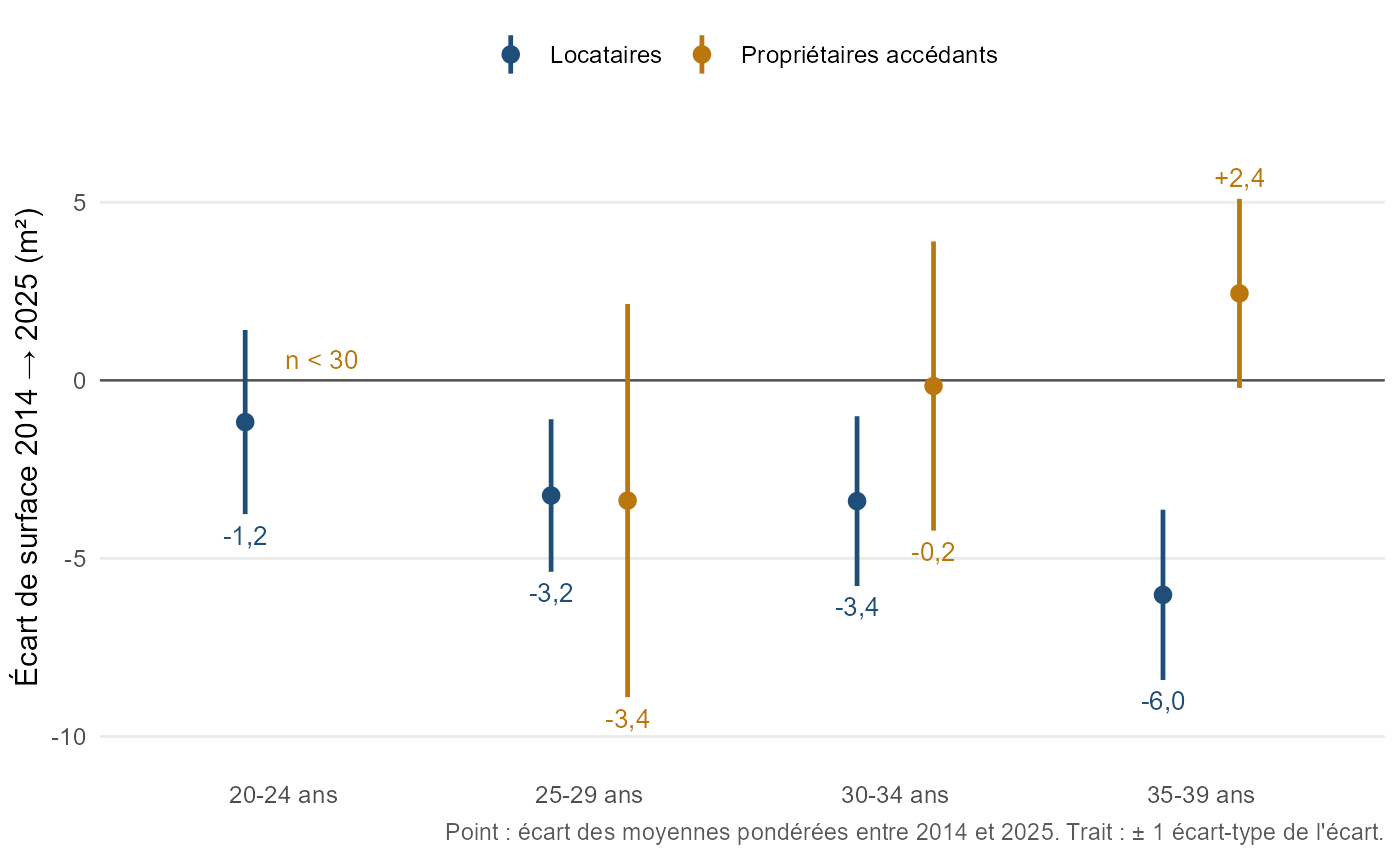
\includegraphics[width=0.88\linewidth]{graph_age_ecart_surface}
\caption{Évolution de la surface du logement des ménages de 20 à 39 ans entre 2014 et 2025, par classe d'âge}\label{fig:age}
\par\vspace{0.2em}
\begin{minipage}{0.88\linewidth}\scriptsize
\textit{Champ} : ménages dont la personne de référence a de 20 à 39 ans, locataires et propriétaires accédants, France entière. \textit{Lecture} : entre 2014 et 2025, la surface moyenne des logements des locataires de 35-39 ans a reculé de 6,0 m² ; le trait représente plus ou moins un écart-type de cet écart. \textit{Méthode} : écart des moyennes pondérées des vagues 2014 et 2025, traitées comme deux échantillons indépendants. Moins de 30 observations : écart non calculé. Quatre ménages déclarant une mensualité supérieure à 10\,000 € sont écartés. \textit{Source} : Insee, SRCV 2014 et 2025 ; calculs de l'auteur.
\end{minipage}
\end{figure}

\begin{figure}[htbp]
\centering
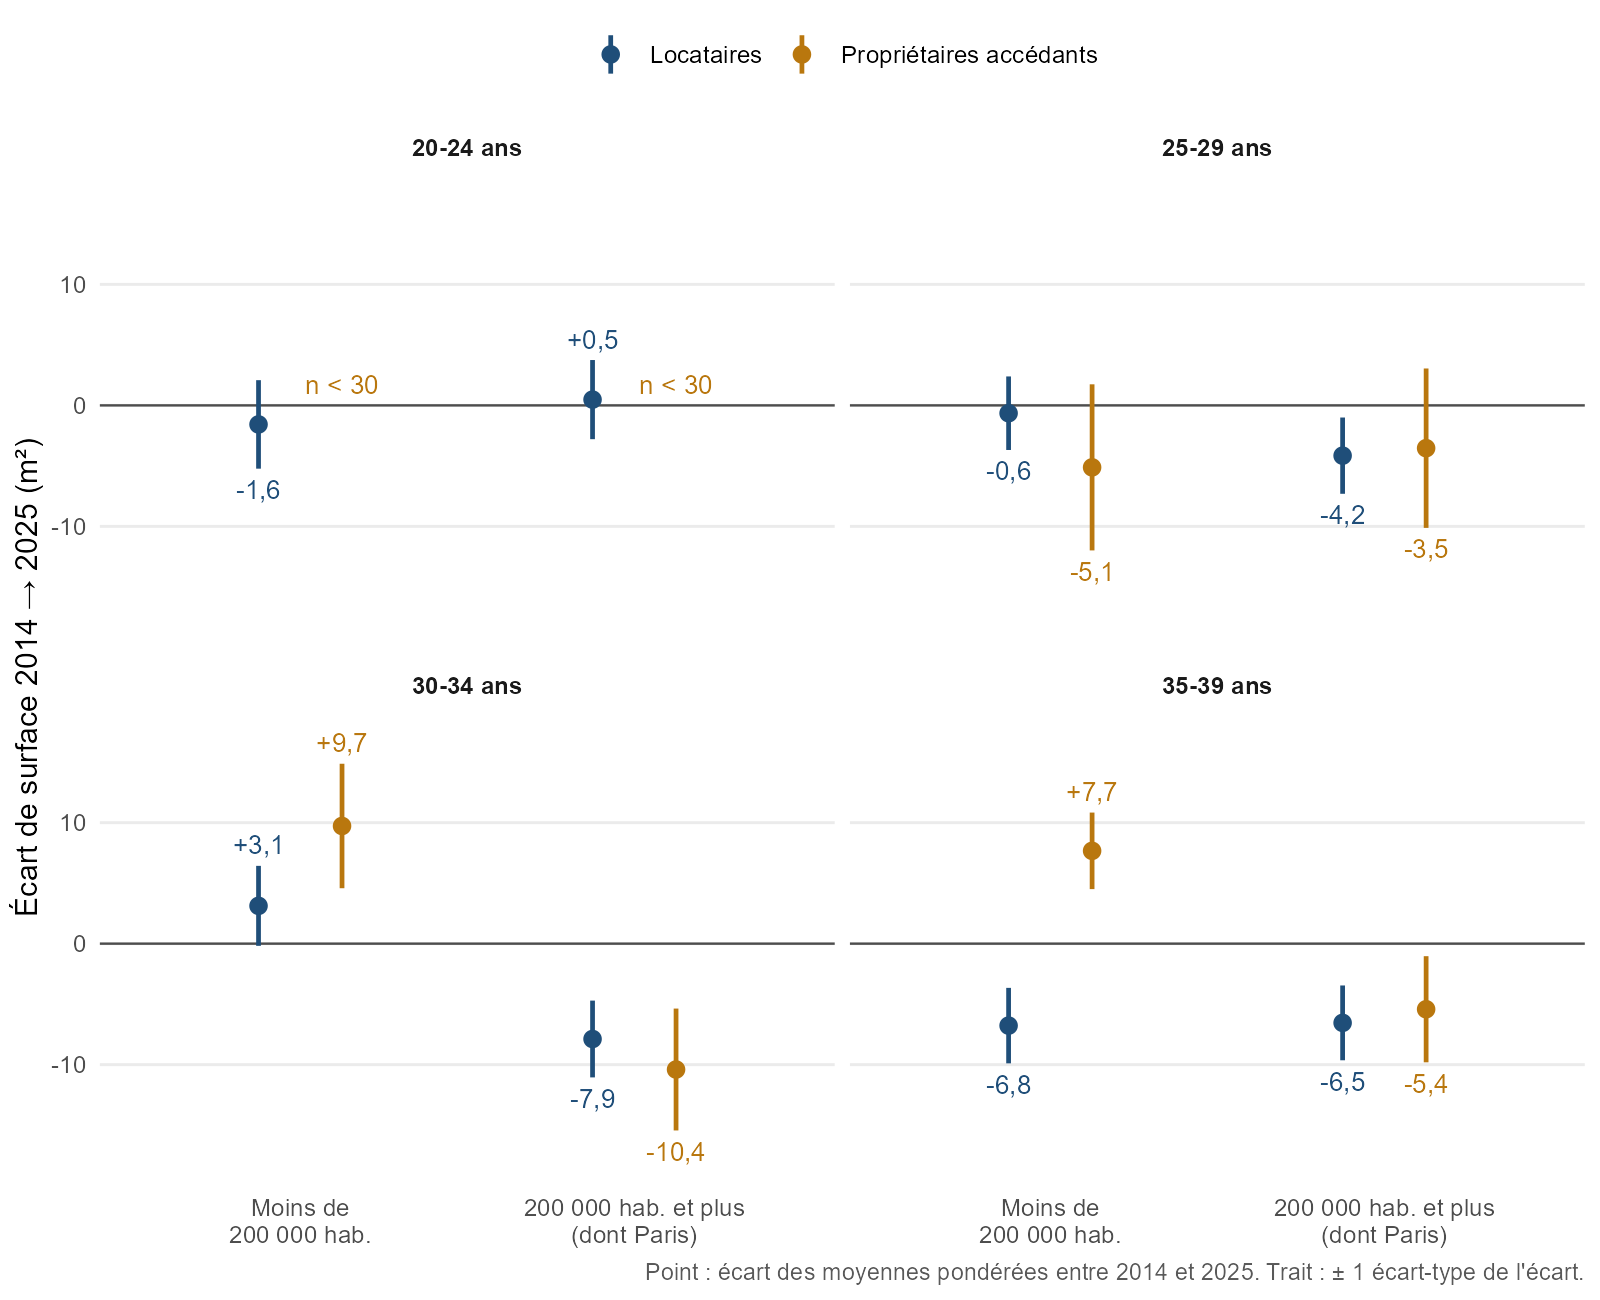
\includegraphics[width=0.88\linewidth]{graph_age_densite_ecart_surface}
\caption{Évolution de la surface du logement entre 2014 et 2025, par classe d'âge et taille d'unité urbaine}\label{fig:age_densite}
\par\vspace{0.2em}
\begin{minipage}{0.88\linewidth}\scriptsize
\textit{Champ, méthode et source} : voir graphique~\ref{fig:age}. Les cinq tranches d'unité urbaine sont regroupées en deux, faute d'effectifs suffisants par classe d'âge : moins de 200\,000 habitants (communes rurales comprises) et 200\,000 habitants ou plus (agglomération parisienne comprise).
\end{minipage}
\end{figure}

% =====================================================================
\section{Résultats}\label{sec:resultats}

\subsection{La surface, pas son prix (P1 et P2)}\label{sec:surface}

Le tableau~\ref{tab:surface} donne les effets de la surface, du coût au mètre carré et du niveau de vie. Dix mètres carrés supplémentaires sont associés à une probabilité de naissance supérieure de 0,34 point, sur un taux de référence de 8,2\,\% : une hausse relative de 4,1\,\%\footnote{Ces effets ne tiennent pas au choix des contrôles d'âge et de géographie. Ajouter l'âge du conjoint et son carré les porte à 0,36 point pour l'ensemble et 0,65 point pour le premier enfant ; retirer le degré d'urbanisation les ramène à 0,31 et 0,58 point.}. L'effet relatif est le même pour le premier enfant (0,59 point sur 13,8\,\%, soit 4,3\,\%) et pour les naissances suivantes (0,30 point sur 6,3\,\%, soit 4,7\,\%). Le coût au mètre carré, en revanche, n'a d'effet dans aucun échantillon : à surface donnée, payer son mètre carré plus cher ne change pas la probabilité d'une naissance. Les prédictions P1 et P2 se vérifient.

\begin{table}[htbp]
\centering\small
\begin{threeparttable}
\caption{Surface, coût au mètre carré et niveau de vie : effets marginaux moyens sur la probabilité de naissance}\label{tab:surface}
\begin{tabular}{@{}lccc@{}}
\toprule
& Ensemble & Premier enfant & Rang 2 et plus \\
\midrule
\multicolumn{4}{@{}l}{\textit{A. Tous les couples}} \\
Surface (+10 m²)                 & 0,34\sym{***} & 0,59\sym{**} & 0,30\sym{***} \\
                                 & (0,08) & (0,20) & (0,08) \\
Coût au m² (+1 € par mois)       & $-$0,06 & $-$0,10 & 0,03 \\
                                 & (0,04) & (0,09) & (0,05) \\
Niveau de vie (+10\,000 € par an) & $-$0,28 & $-$0,16 & $-$0,44\sym{*} \\
                                 & (0,18) & (0,46) & (0,21) \\
Observations                     & 19\,645 & 4\,357 & 15\,288 \\
Naissances                       & 1\,519 & 607 & 912 \\
Taux de naissance (\%)           & 8,2 & 13,8 & 6,3 \\
\addlinespace
\multicolumn{4}{@{}l}{\textit{B. Couples installés depuis au moins trois ans}} \\
Surface (+10 m²)                 & 0,26\sym{***} & 0,35 & 0,26\sym{***} \\
                                 & (0,08) & (0,24) & (0,08) \\
Coût au m² (+1 € par mois)       & $-$0,02 & $-$0,04 & 0,04 \\
                                 & (0,04) & (0,12) & (0,05) \\
Niveau de vie (+10\,000 € par an) & $-$0,20 & $-$0,12 & $-$0,33\sym{\dag} \\
                                 & (0,17) & (0,55) & (0,18) \\
Observations                     & 16\,006 & 2\,645 & 13\,361 \\
Naissances                       & 1\,063 & 368 & 695 \\
Taux de naissance (\%)           & 7,0 & 13,6 & 5,4 \\
\addlinespace
\multicolumn{4}{@{}l}{\textit{C. Couples installés depuis moins de trois ans}} \\
Surface (+10 m²)                 & 0,67\sym{**} & & \\
                                 & (0,21) & & \\
Observations / naissances        & 3\,637 / 456 & & \\
\bottomrule
\end{tabular}
\begin{tablenotes}\scriptsize
\item \sym{***} $p<0{,}001$ ; \sym{**} $p<0{,}01$ ; \sym{*} $p<0{,}05$ ; \sym{\dag} $p<0{,}10$. Erreurs-types entre parenthèses, regroupées au niveau du ménage.
\item \textit{Champ} : couples dont la femme a de 15 à 49 ans, France entière, vagues 2014, 2018 et 2022 à 2025. Le rang est défini avant la naissance.
\item \textit{Modèle} : probit pondéré, effets marginaux moyens en points de pourcentage. Contrôles : statut d'occupation, âge de la femme et son carré, déménagement dans l'année, catégorie socioprofessionnelle, degré d'urbanisation, ZEAT, effets fixes d'année ; pour les rangs deux et plus et l'ensemble, nombre d'enfants et taille du ménage avant la naissance. Coût et niveau de vie en euros constants de 2025 ; niveau de vie hors prestations familiales, minima sociaux et aides au logement, par UC avant la naissance.
\item \textit{Lecture} : dix mètres carrés supplémentaires sont associés à une probabilité de première naissance supérieure de 0,59 point, sur un taux de 13,8\,\%.
\item \textit{Source} : Insee, SRCV ; calculs de l'auteur.
\end{tablenotes}
\end{threeparttable}
\end{table}

L'association n'est pas qu'un effet de déménagements motivés par l'enfant, mais elle en porte la trace. Restreindre l'échantillon aux couples installés depuis au moins trois ans réduit l'effet d'un quart (0,26 contre 0,34 point), sans l'annuler (panneau B). Chez les couples arrivés depuis moins de trois ans, il atteint 0,67 point, plus de deux fois et demie celui des installés (panneau C). Parmi les couples déjà parents, 25,8\,\% de ceux qui déclarent une naissance ont emménagé depuis moins de trois ans, contre 13,5\,\% des autres. Pour le premier enfant, l'effet linéaire chez les installés n'est plus significatif (0,35 point, $p = 0{,}15$) ; la section suivante montre que c'est la forme linéaire qui est en cause, non l'association.

Enfin, l'effet de la surface est plus fort pour le premier enfant que pour les suivants : dans un modèle unique où il varie selon le rang, il vaut 0,90 point pour le premier enfant et 0,20 pour les suivants, et l'écart est significatif ($p = 0{,}018$).

\subsection{Un seuil plutôt qu'une pente (P5)}\label{sec:seuil}

Le modèle prédit une relation concave : l'élasticité de la fécondité à la surface décroît avec la surface. Les données vont plus loin : la relation prend la forme d'une marche (tableau~\ref{tab:seuil}). Par rapport aux couples logés entre 70 et 89 m², ceux qui vivent dans moins de 50 m² ont une probabilité de première naissance inférieure de 9,1 points, deux tiers du taux de référence ; au-delà de 70 m², la surface ne départage plus rien. La marche concerne le premier enfant : pour les naissances suivantes, l'écart sous 50 m² n'est que de 1,7 point, et non significatif. Elle survit à la restriction aux couples installés ($-9{,}1$ points), ce qui explique l'effet linéaire non significatif de la section précédente : chez les couples sans enfant installés, l'association est tout entière concentrée sous le seuil.

\begin{table}[htbp]
\centering\small
\begin{threeparttable}
\caption{Surface en tranches : écart de probabilité de naissance par rapport aux couples logés entre 70 et 89 m²}\label{tab:seuil}
\begin{tabular}{@{}lcccc@{}}
\toprule
& Ensemble & \multicolumn{2}{c}{Premier enfant} & Rang 2 et plus \\
\cmidrule(lr){3-4}
& & Tous & Installés & \\
\midrule
\multicolumn{5}{@{}l}{\textit{A. Quatre tranches}} \\
Moins de 50 m²  & $-$5,80\sym{***} & $-$9,06\sym{***} & $-$9,13\sym{***} & $-$1,68 \\
                & (0,84) & (1,92) & (2,60) & (1,89) \\
50 à 69 m²      & $-$2,23\sym{**} & $-$2,44 & $-$3,87 & $-$1,48\sym{\dag} \\
                & (0,77) & (1,91) & (2,48) & (0,77) \\
90 à 119 m²     & 0,77 & 3,69\sym{\dag} & 2,51 & 0,25 \\
                & (0,80) & (2,20) & (2,84) & (0,75) \\
120 m² et plus  & 0,59 & 2,08 & $-$1,68 & 0,62 \\
                & (0,91) & (2,55) & (3,06) & (0,89) \\
\addlinespace
\multicolumn{5}{@{}l}{\textit{B. Tranches fines sous 70 m²}} \\
Moins de 40 m²  & $-$7,77\sym{***} & $-$12,04\sym{***} & $-$13,14\sym{***} & \\
                & (0,69) & (1,91) & (2,47) & \\
40 à 49 m²      & $-$4,82\sym{***} & $-$8,25\sym{***} & $-$8,06\sym{**} & \\
                & (1,05) & (2,16) & (2,89) & \\
50 à 59 m²      & $-$4,21\sym{***} & $-$6,69\sym{**} & $-$6,87\sym{*} & \\
                & (0,92) & (2,19) & (3,02) & \\
60 à 69 m²      & $-$1,27 & 0,20 & $-$2,38 & \\
                & (0,89) & (2,24) & (2,78) & \\
\addlinespace
Observations    & 19\,645 & 4\,357 & 2\,645 & 15\,288 \\
Taux de naissance (\%) & 8,2 & 13,8 & 13,6 & 6,3 \\
\bottomrule
\end{tabular}
\begin{tablenotes}\scriptsize
\item \sym{***} $p<0{,}001$ ; \sym{**} $p<0{,}01$ ; \sym{*} $p<0{,}05$ ; \sym{\dag} $p<0{,}10$. Erreurs-types entre parenthèses.
\item \textit{Champ, modèle et source} : voir tableau~\ref{tab:surface} ; la surface entre en tranches à la place de la variable continue. Installés : couples dans leur logement depuis au moins trois ans. Dans le panneau B, les tranches de 90 m² et plus sont conservées dans le modèle et non reportées.
\item \textit{Lecture} : les couples sans enfant logés dans moins de 50 m² ont une probabilité de première naissance inférieure de 9,06 points à celle des couples logés entre 70 et 89 m².
\end{tablenotes}
\end{threeparttable}
\end{table}

Le panneau B situe la marche. Pour le premier enfant, l'écart est de 12 points sous 40 m², de 8 points entre 40 et 49 m², de 7 points entre 50 et 59 m², et nul entre 60 et 69 m². Une recherche systématique du point de rupture, qui estime le modèle avec une indicatrice « surface inférieure à $c$ » pour $c$ allant de 35 à 75 m², donne une déviance minimale à 55 m² sur l'ensemble des couples sans enfant et à 45 m² chez les installés, avec un profil presque plat entre 45 et 60 m². Le seuil se situe donc entre 45 et 60 m², sans qu'il soit possible de le localiser plus finement, et il ne tient pas au choix des bornes.

La concavité prédite par le modèle se vérifie donc, sous une forme plus abrupte que la fonction lisse $\nu$ ne le permet. La seconde moitié de P5 ne se vérifie pas. Le modèle prédit que les ménages modestes, logés plus petit, sont les plus sensibles à la surface. Estimé par tercile de niveau de vie, l'effet de dix mètres carrés vaut au contraire 0,21 point dans le tercile le plus modeste ($p = 0{,}06$), 0,33 dans le deuxième et 0,40 dans le plus aisé, et l'égalité des trois ne peut être rejetée ($p = 0{,}31$) ; pour le premier enfant, 0,39, 0,53 et 0,68 point ($p = 0{,}71$). Par tranche d'unité urbaine, l'effet croît des communes rurales (0,18 point, non significatif) à l'agglomération parisienne (0,59 point, $p = 0{,}002$), là où les logements sont les plus petits, comme le voudrait la concavité, mais l'écart n'est pas significatif ($p = 0{,}40$).

\subsection{Une pièce plutôt que des mètres carrés}\label{sec:pieces}

Un seuil entre 45 et 60 m² évoque une indivisibilité : pour accueillir un enfant, il faut une chambre de plus. La norme de peuplement de l'Insee permet de la mesurer directement. Elle attribue à chaque ménage une pièce de séjour, une pièce par couple, une pièce par autre personne de 19 ans ou plus et, pour les moins de 19 ans, une pièce pour deux enfants s'ils ont moins de 7 ans ou sont de même sexe, une pièce par enfant sinon. Pour chaque couple, nous calculons, avant la naissance éventuelle, le nombre de pièces que requiert la norme, et vérifions qu'un enfant de plus, quel que soit son sexe, pourrait y être logé, dans une pièce libre ou dans la chambre d'un frère ou d'une sœur. Les couples se répartissent alors en trois situations : ceux qui ont la place d'un enfant de plus, ceux qui ne l'ont pas, et ceux à qui il manque déjà une pièce. Pour un couple sans enfant vivant seul, la norme se réduit au nombre de pièces : un studio ne suffit pas au couple, un deux-pièces ne laisse pas de place pour un enfant, il en faut trois.

\begin{table}[htbp]
\centering\small
\setlength{\tabcolsep}{4pt}
\begin{threeparttable}
\caption{Place pour un enfant de plus selon la norme de peuplement : répartition des couples, taux de naissance et effets marginaux moyens}\label{tab:pieces}
\begin{tabular}{@{}lcccccc@{}}
\toprule
& \multicolumn{3}{c}{Premier enfant} & \multicolumn{3}{c}{Rang 2 et plus} \\
\cmidrule(lr){2-4}\cmidrule(lr){5-7}
\multicolumn{7}{@{}l}{\textit{A. Répartition des couples et taux de naissance}} \\
& Part (\%) & \shortstack{Surface\\médiane (m²)} & Taux (\%) & Part (\%) & \shortstack{Surface\\médiane (m²)} & Taux (\%) \\
\cmidrule(lr){2-4}\cmidrule(lr){5-7}
Place pour un enfant de plus & 73,5 & 84 & 18,6 & 79,7 & 110 & 8,0 \\
Pas de place                 & 23,4 & 47 & 7,7  & 12,3 & 80  & 4,2 \\
Il manque déjà une pièce     & 3,1  & 29 & 2,4  & 8,0  & 70  & 6,5 \\
\addlinespace
\multicolumn{7}{@{}l}{\textit{B. Effets marginaux moyens (points) ; référence : place pour un enfant de plus}} \\
& (1) & (2) & (3) & (4) & (5) & (6) \\
\cmidrule(lr){2-4}\cmidrule(lr){5-7}
Pas de place             & $-$10,17\sym{***} & $-$9,88\sym{***} & $-$7,96\sym{***} & $-$2,11\sym{**} & $-$1,81\sym{*} & $-$2,08\sym{**} \\
                         & (1,46) & (1,50) & (2,02) & (0,77) & (0,79) & (0,78) \\
Il manque déjà une pièce & $-$13,00\sym{***} & $-$12,78\sym{***} & $-$11,35\sym{***} & $-$1,80\sym{*} & $-$1,38 & $-$1,58 \\
                         & (2,15) & (2,21) & (2,69) & (0,88) & (0,92) & (0,98) \\
Surface (+10 m²)         & & 0,22 & & & 0,26\sym{**} & \\
                         & & (0,21) & & & (0,08) & \\
Moins de 60 m²           & & & $-$4,50\sym{*} & & & $-$0,75 \\
                         & & & (2,26) & & & (1,29) \\
Observations             & 4\,336 & 4\,336 & 4\,336 & 15\,192 & 15\,192 & 15\,192 \\
Taux de naissance (\%)   & \multicolumn{3}{c}{13,8} & \multicolumn{3}{c}{6,3} \\
\bottomrule
\end{tabular}
\begin{tablenotes}\scriptsize
\item \sym{***} $p<0{,}001$ ; \sym{**} $p<0{,}01$ ; \sym{*} $p<0{,}05$. Erreurs-types entre parenthèses, regroupées au niveau du ménage.
\item \textit{Norme de peuplement} : une pièce de séjour, une pièce par couple, une pièce par autre personne de 19 ans ou plus ; pour les moins de 19 ans, une pièce pour deux enfants s'ils ont moins de 7 ans ou sont de même sexe, une pièce par enfant sinon. Composition du ménage avant la naissance, nouveau-né exclu. Un couple a la place d'un enfant de plus si un enfant supplémentaire, quel que soit son sexe, peut être logé selon la norme, dans une pièce libre ou dans la chambre d'un autre enfant.
\item \textit{Champ} : couples dont la femme a de 15 à 49 ans ; panneau A, vagues 2014, 2018, 2024 et 2025, moyennes pondérées (les vagues 2022 et 2023 sont écartées en raison de l'anomalie de pondération) ; panneau B, toutes les vagues.
\item \textit{Modèle} : spécification du tableau~\ref{tab:surface}, la place disponible remplaçant la surface (colonnes 1 et 4), puis s'ajoutant à la surface (2 et 5) ou à une indicatrice de logement de moins de 60 m² (3 et 6).
\item \textit{Lecture} : 23,4\,\% des couples sans enfant n'ont pas la place d'un enfant ; leur probabilité de première naissance est inférieure de 10,17 points à celle des couples qui l'ont, à caractéristiques données.
\item \textit{Source} : Insee, SRCV ; calculs de l'auteur.
\end{tablenotes}
\end{threeparttable}
\end{table}

Près d'un quart des couples sans enfant n'ont pas la place d'un enfant, et 3\,\% n'ont qu'une pièce (tableau~\ref{tab:pieces}). Leur surface médiane est de 47 et 29 m², contre 84 m² pour ceux qui ont la place, et leur taux de première naissance de 7,7 et 2,4\,\%, contre 18,6\,\%. À caractéristiques données, ne pas avoir la place d'un enfant abaisse la probabilité de première naissance de 10,2 points, n'avoir qu'une pièce de 13,0 points (colonne 1). Surtout, la place absorbe l'effet de la surface : à place donnée, dix mètres carrés de plus n'ont plus d'effet significatif sur la première naissance (0,22 point, contre 0,59 sans la place ; colonne 2). Une indicatrice de logement de moins de 60 m² garde un effet propre, plus faible ($-4{,}5$ points, $p = 0{,}05$), quand l'absence de place reste à $-8{,}0$ points (colonne 3). Le seuil du premier enfant est d'abord un seuil en pièces : celui du trois-pièces.

Aux rangs suivants, le manque de place compte aussi, mais moins : $-2{,}1$ points pour les parents qui n'ont pas la place d'un enfant de plus, $-1{,}8$ pour ceux à qui il manque déjà une pièce, soit environ un tiers du taux de naissance. La surface y garde son effet à place donnée (0,26 point), et le seuil de 60 m² n'en a pas : pour les naissances de rang deux ou plus, la relation reste une pente plutôt qu'une marche.

Le recensement confirme ces résultats avec une tout autre précision (annexe~\ref{app:rp}, tableaux~\ref{tab:rp_place} à \ref{tab:rp_coupe}). Sur les 614\,000 couples sans enfant du recensement de 2019, la répartition entre les trois situations est presque la même que dans SRCV (73, 23 et 4\,\% en 2019). Le taux de première naissance est de 6,3 à 6,4\,\% sous 40 m², de 8,9\,\% entre 40 et 59 m², de 14,7\,\% entre 60 et 79 m², et ne varie plus au-delà. À caractéristiques données, ne pas avoir la place d'un enfant l'abaisse de 9,3 points en 2019 et de 7,3 points en 2023, contre 10,2 dans SRCV. Lorsque la place et la surface entrent ensemble, chacune garde un effet propre, comme dans la colonne 3 du tableau~\ref{tab:pieces} : la marche du premier enfant est d'abord celle du trois-pièces, que la surface prolonge.

Ces situations ont progressé dans SRCV sur la période. La part des couples sans enfant qui n'ont pas la place d'un enfant, ou à qui une pièce manque déjà, est passée de 24,0\,\% en 2014 à 27,4\,\% en 2025 ; celle des parents à qui il manque déjà une pièce a presque doublé, de 5,6 à 10,5\,\%. Le recensement ne confirme pas cette dégradation entre 2019 et 2023 : la première part y recule de 26,9 à 24,5\,\%, la seconde progresse de 8,0 à 8,8\,\% seulement.

\subsection{Le revenu (P3)}\label{sec:revenu}

Selon le modèle, le revenu n'agit sur la fécondité qu'à travers la surface : le salaire du jeune adulte détermine la surface achetée, et celui de l'adulte n'entre pas dans la décision d'enfant. À surface donnée, le revenu ne devrait donc pas avoir d'effet. Le tableau~\ref{tab:revenu} confronte cette prédiction à deux mesures du niveau de vie.

\begin{table}[htbp]
\centering\small
\begin{threeparttable}
\caption{Effet du niveau de vie sans puis avec contrôle de la surface, selon la mesure du niveau de vie}\label{tab:revenu}
\begin{tabular}{@{}lcccc@{}}
\toprule
& \multicolumn{2}{c}{Ensemble} & \multicolumn{2}{c}{Premier enfant} \\
\cmidrule(lr){2-3}\cmidrule(lr){4-5}
& Sans surface & Avec surface & Sans surface & Avec surface \\
\midrule
\multicolumn{5}{@{}l}{\textit{A. Niveau de vie avant la naissance, hors transferts}} \\
Niveau de vie (+10\,000 €) & $-$0,09 & $-$0,28 & 0,05 & $-$0,16 \\
                         & (0,17) & (0,18) & (0,44) & (0,46) \\
Surface (+10 m²)         & & 0,34\sym{***} & & 0,59\sym{**} \\
                         & & (0,08) & & (0,20) \\
\addlinespace
\multicolumn{5}{@{}l}{\textit{B. Niveau de vie usuel : revenu disponible par UC}} \\
Niveau de vie (+10\,000 €) & $-$2,24\sym{***} & $-$2,59\sym{***} & $-$4,18\sym{***} & $-$4,49\sym{***} \\
                         & (0,33) & (0,33) & (0,74) & (0,75) \\
Surface (+10 m²)         & & 0,53\sym{***} & & 0,87\sym{***} \\
                         & & (0,08) & & (0,21) \\
\addlinespace
Observations             & \multicolumn{2}{c}{19\,645} & \multicolumn{2}{c}{4\,357} \\
\bottomrule
\end{tabular}
\begin{tablenotes}\scriptsize
\item \sym{***} $p<0{,}001$ ; \sym{**} $p<0{,}01$. Erreurs-types entre parenthèses.
\item \textit{Champ, modèle et source} : voir tableau~\ref{tab:surface}. Toutes les spécifications contrôlent le coût au mètre carré. Panneau A : revenu disponible hors prestations familiales, minima sociaux et aides au logement, rapporté aux unités de consommation avant la naissance. Panneau B : revenu disponible rapporté aux unités de consommation du ménage telles qu'enregistrées, nouveau-né compris.
\end{tablenotes}
\end{threeparttable}
\end{table}

Mesuré avant la naissance, le niveau de vie n'a pas d'effet significatif, ni sans contrôle de la surface ($-0{,}09$ point pour 10\,000 €, $p = 0{,}59$), ni avec ($-0{,}28$ point, $p = 0{,}13$), et il n'en a aucun pour le premier enfant. L'introduction de la surface abaisse le coefficient du revenu de 0,19 point : c'est la part de l'effet du revenu qui passe par la surface, positive comme le prédit le modèle. Mais l'effet total n'est pas positif, ce qui suppose un effet direct légèrement négatif à surface donnée, non significatif sur l'ensemble et pour le premier enfant, à la limite de la significativité pour les naissances de rang deux ou plus ($-0{,}44$ point, $p = 0{,}04$ ; tableau~\ref{tab:surface}). P3 se vérifie pour l'essentiel : à surface donnée, le revenu ne compte guère.

Ce résultat dépend entièrement de la mesure. Avec le niveau de vie usuel (panneau B), le revenu paraît peser fortement et négativement sur la natalité, neuf fois plus que dans le panneau A, et plus encore pour le premier enfant. Cet effet est fabriqué par la naissance elle-même : le nouveau-né ajoute des unités de consommation au dénominateur et déclenche des transferts au numérateur. Le biais se propage à la surface, dont l'effet est surestimé de plus de moitié (0,53 contre 0,34 point) lorsque le revenu est mal mesuré. Toute analyse qui rapproche fécondité et niveau de vie courant est exposée à ce mécanisme.

\subsection{L'ordre temporel (P4)}\label{sec:panel}

P4 est la seule prédiction qui départage les deux lectures du lien entre logement et naissances. Si le logement contraint la fécondité, la surface acquise doit prédire les naissances \emph{à venir}. Si le logement est choisi en vue d'un projet d'enfant, la surface est associée aux naissances récentes ou en cours, sans prédire nécessairement les suivantes.

Le panel des vagues 2022 à 2025 permet de suivre 7\,184 observations de couples d'une vague à la suivante (de 2022 à 2023, de 2023 à 2024 et de 2024 à 2025). La naissance entre $t$ et $t+1$ est l'apparition dans le ménage, en $t+1$, d'un enfant né en $t$ ou $t+1$ et absent en $t$. Pour isoler l'effet de l'ordre temporel, nous estimons exactement la spécification de la coupe sur l'échantillon du panel, en ne changeant que la naissance expliquée (tableau~\ref{tab:panel}).

\begin{table}[htbp]
\centering\small
\begin{threeparttable}
\caption{Coupe et panel : effet de dix mètres carrés sur la naissance contemporaine et sur la naissance suivante}\label{tab:panel}
\begin{tabular}{@{}lccc@{}}
\toprule
& Tous les couples & Installés & \shortstack{Premier enfant,\\installés} \\
\midrule
\multicolumn{4}{@{}l}{\textit{Coupe des vagues 2022 à 2024, naissance en $t$}} \\
Surface (+10 m²) & 0,30\sym{***} & 0,23\sym{**} & 0,38 \\
                 & (0,08) & (0,08) & (0,30) \\
Observations / naissances & 10\,402 / 771 & 8\,549 / 545 & 1\,419 / 190 \\
\addlinespace
\multicolumn{4}{@{}l}{\textit{(a) Échantillon du panel, naissance en $t$}} \\
Surface (+10 m²) & 0,31\sym{**} & 0,26\sym{**} & 0,28 \\
                 & (0,10) & (0,10) & (0,38) \\
Observations / naissances & 7\,184 / 526 & 5\,963 / 378 & 1\,014 / 139 \\
\addlinespace
\multicolumn{4}{@{}l}{\textit{(b) Échantillon du panel, naissance entre $t$ et $t+1$}} \\
Surface (+10 m²) & 0,26\sym{*} & 0,09 & $-$0,36 \\
                 & (0,11) & (0,12) & (0,35) \\
Observations / naissances & 7\,184 / 395 & 5\,963 / 272 & 875 / 84 \\
\bottomrule
\end{tabular}
\begin{tablenotes}\scriptsize
\item \sym{***} $p<0{,}001$ ; \sym{**} $p<0{,}01$ ; \sym{*} $p<0{,}05$. Erreurs-types entre parenthèses.
\item \textit{Champ} : couples dont la femme a de 15 à 49 ans, vagues 2022 à 2024 ; échantillon du panel : couples observés en $t$ et en $t+1$. Installés : dans leur logement depuis au moins trois ans en $t$.
\item \textit{Modèle} : spécification du tableau~\ref{tab:surface}, identique dans les trois blocs ; seule change la naissance expliquée. En (b), le rang et les contrôles de composition sont ceux observés en $t$.
\item \textit{Source} : Insee, SRCV 2022-2025 ; calculs de l'auteur.
\end{tablenotes}
\end{threeparttable}
\end{table}

L'échantillon du panel n'a rien de particulier : la naissance en $t$ y est associée à la surface comme dans la coupe complète (bloc (a)). La naissance suivante ne l'est pas chez les couples installés : l'effet tombe à 0,09 point, le tiers de l'effet contemporain sur les mêmes observations, et n'est pas significatif ($p = 0{,}44$). Chez les couples sans enfant installés, le signe s'inverse ($-0{,}36$ point, non significatif). Sur l'ensemble des couples, l'effet prospectif subsiste (0,26 point, $p = 0{,}02$), mais il est porté par des couples arrivés récemment dans leur logement, ce qui est la signature d'un déménagement en vue de l'enfant.

Le panel annuel est court, et l'estimation imprécise. L'intervalle de confiance à 95\,\% de l'effet prospectif chez les installés, $[-0{,}14\,;\,0{,}31]$, contient l'effet contemporain de 0,26 point, et l'effet minimal détectable à 5\,\% avec une puissance de 80\,\% est de 0,32 point. Tester l'égalité de l'effet prospectif à l'effet contemporain, en traitant ce dernier comme connu, donne $p \approx 0{,}13$. Sur ce seul test, la prédiction centrale du modèle n'est pas réfutée ; elle n'est pas vérifiée non plus. Trois prolongements permettent d'aller plus loin : allonger l'horizon, mesurer la place disponible en pièces plutôt qu'en mètres carrés, et regarder l'ordre dans lequel surviennent agrandissements et naissances.

\paragraph{Un horizon plus long.} Le test annuel ne voit que la naissance de l'année suivante. Or une partie des ménages de 2014 est réinterrogée en 2018, et une partie de ceux de 2022 l'est jusqu'en 2025. En suivant chaque couple de sa première à sa dernière observation dans l'un de ces deux groupes, on compte toutes les naissances survenues entre les deux, sur un horizon d'un à quatre ans : 5\,849 couples, dont 750 connaissent au moins une naissance après la vague de base, et 501 parmi les installés, contre 272 dans le test annuel. La spécification est celle de la coupe, avec la parité observée à la vague de base, une indicatrice de naissance à cette vague et des effets fixes croisant la vague de base et l'horizon de suivi. Les taux de naissance différant selon l'horizon, nous comparons les effets en proportion du taux (tableau~\ref{tab:horizon}, panneau A).

Le résultat annuel se confirme. Chez les couples installés, dix mètres carrés sont associés à une probabilité de naissance contemporaine supérieure de 2,8\,\% du taux, et à des naissances suivantes plus probables de 1,2\,\% seulement, effet non significatif ($p = 0{,}42$). Le profil est le même dans les deux groupes de panel (0,09 point de 2014 à 2018, 0,10 de 2022 à 2025). Chez les couples sans enfant, l'écart est plus net : un logement de moins de 60 m² est associé à une probabilité de première naissance contemporaine inférieure de 71\,\%, mais ne réduit les naissances des années suivantes que de 13\,\%, écart non significatif dont l'intervalle de confiance, de $-43$ à $+17\,\%$ du taux, exclut l'effet contemporain. Le gain de précision reste limité pour la surface continue : l'effet minimal détectable, rapporté au taux, passe de 7 à 4\,\%, au-dessus de l'effet contemporain.

\paragraph{La place en pièces.} La section~\ref{sec:pieces} a montré qu'en coupe, la place disponible pour un enfant de plus, mesurée par la norme de peuplement, absorbe l'effet de la surface au premier enfant. Le test prospectif donne avec cette mesure un résultat différent (tableau~\ref{tab:horizon}, panneau B). Pour les naissances suivantes, la place est mesurée à la vague de base avec la composition du ménage observée à cette date, nouveau-né éventuel compris. Les couples sans enfant qui n'ont pas la place d'un enfant ont une probabilité de première naissance contemporaine inférieure de 71\,\% du taux ; leurs naissances des années suivantes sont encore inférieures de 35\,\% ($p = 0{,}01$). Chez les parents, c'est la pièce qui manque déjà qui pèse : $-54\,\%$ sur la naissance contemporaine, $-39\,\%$ sur les suivantes ($p = 0{,}01$). Mesurée en pièces, la contrainte prédit donc les naissances à venir, avec un effet réduit de moitié environ pour le premier enfant et d'un quart pour les suivants.

\begin{table}[htbp]
\centering\small
\begin{threeparttable}
\caption{Naissance à la vague de base et naissances des années suivantes, sur les mêmes couples : panel à horizon long}\label{tab:horizon}
\begin{tabular}{@{}lcccc@{}}
\toprule
& \multicolumn{2}{c}{\shortstack{Naissance à la\\vague de base}} & \multicolumn{2}{c}{\shortstack{Naissances des\\années suivantes}} \\
\cmidrule(lr){2-3}\cmidrule(lr){4-5}
& Points & \% du taux & Points & \% du taux \\
\midrule
\multicolumn{5}{@{}l}{\textit{A. Surface}} \\
Surface (+10 m²), tous les couples   & 0,32\sym{*} & 3,2 & 0,23 & 1,5 \\
                                     & (0,15) & & (0,19) & \\
Surface (+10 m²), installés          & 0,24\sym{\dag} & 2,8 & 0,15 & 1,2 \\
                                     & (0,14) & & (0,19) & \\
Moins de 60 m², couples sans enfant  & $-$12,20\sym{***} & $-$71 & $-$3,06 & $-$13 \\
                                     & (3,32) & & (3,63) & \\
\addlinespace
\multicolumn{5}{@{}l}{\textit{B. Place pour un enfant de plus selon la norme de peuplement}} \\
Couples sans enfant : pas de place   & $-$12,32\sym{***} & $-$71 & $-$8,35\sym{*} & $-$35 \\
                                     & (3,03) & & (3,25) & \\
\quad il manque déjà une pièce       & $-$9,68 & $-$56 & $-$10,59 & $-$45 \\
                                     & (6,63) & & (8,69) & \\
Parents : pas de place               & $-$2,87\sym{*} & $-$41 & $-$1,01 & $-$7 \\
                                     & (1,29) & & (1,95) & \\
\quad il manque déjà une pièce       & $-$3,81\sym{**} & $-$54 & $-$5,19\sym{**} & $-$39 \\
                                     & (1,35) & & (2,00) & \\
\addlinespace
\multicolumn{5}{@{}l}{\textit{Taux de naissance (\%) ; observations / naissances}} \\
Tous les couples                     & 9,8 & 5\,849 / 512 & 15,8 & 5\,849 / 750 \\
Installés                            & 8,5 & 4\,788 / 371 & 12,9 & 4\,788 / 501 \\
Couples sans enfant                  & 17,3 & 1\,351 / 216 & 23,6 & 1\,135 / 244 \\
Parents                              & 7,0 & 4\,498 / 296 & 13,5 & 4\,714 / 506 \\
\bottomrule
\end{tabular}
\begin{tablenotes}\scriptsize
\item \sym{***} $p<0{,}001$ ; \sym{**} $p<0{,}01$ ; \sym{*} $p<0{,}05$ ; \sym{\dag} $p<0{,}10$. Erreurs-types entre parenthèses, regroupées au niveau du ménage.
\item \textit{Champ} : couples dont la femme a de 15 à 49 ans, suivis de leur première à leur dernière observation dans le groupe de panel 2014-2018 ou 2022-2025 (horizon d'un à quatre ans). Couples sans enfant : sans enfant avant la naissance éventuelle de la vague de base (première colonne), sans enfant à la vague de base (troisième colonne). Installés : dans leur logement depuis au moins trois ans à la vague de base.
\item \textit{Modèle} : spécification du tableau~\ref{tab:surface} ; pour les naissances suivantes, parité observée à la vague de base, indicatrice de naissance à cette vague, effets fixes croisant la vague de base et l'horizon. Naissances suivantes : au moins un enfant présent à la dernière vague, né après la vague de base ou absent du ménage à cette vague. Panneau B : référence, les couples qui ont la place d'un enfant de plus (section~\ref{sec:pieces}) ; panneau A, troisième ligne : référence, 60 m² ou plus. Effectifs : observations / naissances.
\item \textit{Source} : Insee, SRCV 2014, 2018 et 2022-2025 ; calculs de l'auteur.
\end{tablenotes}
\end{threeparttable}
\end{table}

\paragraph{Qui vient en premier ?} Si les couples ont leurs enfants là où ils sont et s'agrandissent ensuite, la naissance doit précéder le déménagement ; s'ils ajustent leur logement à un projet d'enfant, ou attendent d'avoir la place, l'agrandissement doit précéder la naissance. Le panel 2022-2025 permet de suivre des séquences de trois vagues successives, $t-1$, $t$ et $t+1$. Nous appelons agrandissement un déménagement vers un logement plus grand d'au moins 10 m² ou d'une pièce, et comparons deux probabilités : celle d'une naissance entre $t$ et $t+1$ selon que le couple s'est agrandi ou non entre $t-1$ et $t$ ; celle d'un agrandissement entre $t$ et $t+1$ selon qu'une naissance est survenue ou non entre $t-1$ et $t$.

L'agrandissement précède la naissance bien plus qu'il ne la suit. Les couples sans enfant qui viennent de s'agrandir ont une probabilité de première naissance l'année suivante de 18,6\,\%, contre 9,8\,\% pour ceux qui n'ont pas déménagé ($p = 0{,}05$, test exact de Fisher) ; parmi les couples sans enfant logés sous 60 m² en $t-1$, de 24,1\,\% contre 5,8\,\% pour ceux qui ne se sont pas agrandis ($p = 0{,}008$). Chez les parents, 7,5 contre 3,0\,\% ($p = 0{,}06$). À l'inverse, une naissance n'augmente pas significativement la probabilité de s'agrandir l'année suivante : 10,0 contre 7,8\,\% au premier enfant, 4,5 contre 2,6\,\% aux rangs suivants, 12,5 contre 12,0\,\% sous 60 m² ($p$ compris entre 0,29 et 1). Ces proportions ne sont pas pondérées, et les effectifs sont faibles : 59 couples sans enfant s'agrandissent, dont 11 ont ensuite un enfant. Ce profil ne départage pas, à lui seul, contrainte et anticipation, qui prédisent toutes deux que l'on s'agrandit d'abord. Il écarte en revanche un logement qui s'ajusterait après coup à des naissances survenues sans lui.

\paragraph{Au total.} P4 n'est que partiellement vérifiée. Mesurée en mètres carrés, la contrainte ne se retrouve pas dans les naissances à venir, même sur quatre ans ; mesurée en pièces, elle s'y retrouve, avec une ampleur réduite de moitié environ par rapport à la coupe pour le premier enfant. Une partie de l'association transversale tient donc à l'anticipation — les couples s'installent là où ils comptent avoir un enfant, et s'agrandissent avant lui — ; une autre résiste au test d'ordre temporel, et c'est une contrainte d'indivisibilité, celle d'une pièce, plus que de surface. Le recensement, qui ne suit pas les ménages mais date leur emménagement, va dans le même sens : l'effet du manque de place y est le plus fort chez les couples arrivés depuis moins de deux ans, mais il conserve plus des quatre cinquièmes de son ampleur relative chez ceux qui sont installés depuis cinq ans ou plus (annexe~\ref{app:rp}, tableau~\ref{tab:rp_anciennete}).

\subsection{La géographie (P6)}\label{sec:geo}

Étendu à deux régions, le modèle prédit des logements urbains plus petits et plus chers, une fécondité urbaine plus faible, et aucun effet de la ville à surface donnée. Ses deux premières prédictions sont quantitatives : avec $\gamma = 0{,}43$, l'écart de niveau de vie entre une ville et la campagne détermine le rapport des surfaces, $(w_u/w_r)^{-1/\gamma}$, et celui des prix, $(w_u/w_r)^{(1+\gamma)/\gamma}$. Le tableau~\ref{tab:geo} les confronte aux données, par tranche d'unité urbaine, sur les vagues 2014, 2018, 2024 et 2025, les vagues 2022 et 2023 étant écartées des moyennes pondérées en raison de l'anomalie de pondération.

\begin{table}[htbp]
\centering\small
\begin{threeparttable}
\caption{Surfaces, prix et naissances par tranche d'unité urbaine : observé et prédit par le modèle à deux régions}\label{tab:geo}
\begin{tabular}{@{}lcccccc@{}}
\toprule
& \shortstack{Niveau\\de vie (k€)} & \shortstack{Surface\\(m²)} & \shortstack{Surface\\relative} & \shortstack{Prix\\relatif} & \shortstack{Taux de\\naissance (\%)} & \shortstack{Taux de 1\textsuperscript{re}\\naissance (\%)} \\
\midrule
Communes rurales             & 27,5 & 121,9 & 1        & 1        & 9,0  & 18,9 \\
Moins de 20\,000 hab.        & 28,6 & 109,8 & 0,90 [0,91] & 1,13 [1,15] & 9,6  & 17,3 \\
20\,000 à 199\,999 hab.      & 26,7 & 100,5 & 0,82 [1,07] & 1,17 [0,91] & 10,3 & 15,8 \\
200\,000 hab. à 2 millions   & 29,5 & 92,0  & 0,75 [0,85] & 1,39 [1,26] & 9,7  & 12,9 \\
Agglomération de Paris       & 35,3 & 79,8  & 0,65 [0,56] & 2,05 [2,31] & 9,5  & 15,7 \\
\bottomrule
\end{tabular}
\begin{tablenotes}\scriptsize
\item \textit{Champ} : couples dont la femme a de 15 à 49 ans, vagues 2014, 2018, 2024 et 2025 ; moyennes pondérées.
\item \textit{Lecture} : dans l'agglomération parisienne, la surface moyenne vaut 0,65 fois celle des communes rurales, et le coût au mètre carré 2,05 fois. Entre crochets, les rapports prédits par la proposition~\ref{prop:regions} avec $\gamma = 0{,}43$, à partir du rapport des niveaux de vie : 0,56 et 2,31.
\item \textit{Source} : Insee, SRCV ; calculs de l'auteur.
\end{tablenotes}
\end{threeparttable}
\end{table}

Aux deux extrémités, le modèle restitue l'ordre de grandeur : dans l'agglomération parisienne, où le niveau de vie est supérieur de 29\,\% à celui des communes rurales, il prédit des surfaces de 0,56 fois et des prix de 2,31 fois ceux des communes rurales, pour 0,65 et 2,05 observés. Il ne restitue pas le profil intermédiaire : les villes de 20\,000 à 200\,000 habitants ont des logements plus petits que les communes rurales avec un niveau de vie légèrement inférieur, ce qu'un modèle où seule la prime salariale distingue les régions ne peut produire. Les aménités, la structure du parc et la distribution des emplois, absentes du modèle, y suffisent sans doute.

La troisième prédiction échoue. Le taux de naissance ne décroît pas avec la taille de l'unité urbaine : 9,0\,\% dans les communes rurales, 9,5\,\% dans l'agglomération parisienne. Le taux de première naissance est plus faible dans les grandes agglomérations de province (12,9\,\% contre 18,9\,\%), mais l'écart disparaît une fois l'âge et les autres caractéristiques contrôlés : dans le modèle de l'équation~\eqref{eq:probit}, aucun effet de la tranche d'unité urbaine n'est significatif, que la surface soit contrôlée ou non (tests joints : $p = 0{,}96$ et $0{,}64$ sur l'ensemble des couples, $0{,}41$ et $0{,}47$ pour le premier enfant). Or, à l'effet estimé de la surface, les 42 m² qui séparent un logement parisien d'un logement rural devraient y abaisser la probabilité de naissance de 1,4 point. Cet écart ne se voit pas. À surface donnée, l'effet estimé de l'agglomération parisienne est d'ailleurs positif (0,8 point sur l'ensemble, 8,4 points pour le premier enfant), quoique très imprécis. Dans SRCV, l'absence d'effet de la ville à surface donnée se vérifie donc, mais trivialement : la ville n'a pas d'effet du tout.

Le recensement nuance ce constat (annexe~\ref{app:rp}, tableau~\ref{tab:rp_geo}). Il le confirme sur l'ensemble des naissances : en 2019, le taux de naissance des couples est de 7,0\,\% dans les petites communes, de 9,0\,\% dans celles de 20\,000 à 100\,000 habitants et de 8,2\,\% à Paris. Mais le taux de première naissance est plus faible dans les grandes villes : 9,0\,\% à Paris et 10,4\,\% dans les autres communes de 100\,000 habitants ou plus, contre 12,7\,\% dans les petites communes, soit, à caractéristiques données, un écart de $-5{,}0$ et $-3{,}4$ points. Or sept couples sans enfant parisiens sur dix n'ont pas la place d'un enfant, contre moins d'un sur dix dans les petites communes ; une fois la place contrôlée, l'écart parisien disparaît en 2019 et tombe à $-1{,}4$ point en 2023. Aux rangs suivants, la fécondité des grandes communes est au contraire plus élevée. Pour le premier enfant, les deux dernières prédictions de P6 se vérifient donc dans le recensement, alors que SRCV, avec 607 premières naissances, ne permettait pas de les voir ; l'absence d'écart sur l'ensemble des naissances tient aux rangs suivants.

\subsection{Bilan}

Le tableau~\ref{tab:bilan} résume la confrontation. Les prédictions en coupe se vérifient : la surface compte, son prix non, et le revenu ne compte qu'à travers elle. La forme de la relation est plus abrupte que dans le modèle, concentrée sur le premier enfant, et elle se mesure mieux en pièces qu'en mètres carrés. Les deux prédictions qui engagent le mécanisme de contrainte lui-même ne se vérifient qu'en partie : l'ordre temporel, pour la place disponible mesurée en pièces mais non pour la surface ; la géographie, pour les premières naissances seulement, et dans le recensement.

\begin{table}[htbp]
\centering\small
\begin{threeparttable}
\caption{Les prédictions du modèle confrontées aux données}\label{tab:bilan}
\begin{tabular}{@{}p{0.05\linewidth}p{0.36\linewidth}p{0.49\linewidth}@{}}
\toprule
& Prédiction & Résultat \\
\midrule
P1 & La surface élève la probabilité de naissance & Vérifiée : +4\,\% du taux de naissance pour dix mètres carrés, y compris chez les installés \\
P2 & À surface donnée, le prix n'a pas d'effet & Vérifiée : coût au mètre carré sans effet \\
P3 & Le revenu n'agit qu'à travers la surface & Vérifiée pour l'essentiel, à condition de mesurer le revenu avant la naissance \\
P4 & La surface prédit les naissances à venir & Partiellement vérifiée : la surface ne prédit pas les naissances à venir, même sur quatre ans ; le manque de place pour un enfant les prédit, avec un effet réduit de moitié environ par rapport à la coupe ; les agrandissements précèdent les naissances \\
P5 & Concavité ; ménages modestes plus sensibles & Concavité vérifiée, sous la forme d'un seuil entre 45 et 60 m² pour le premier enfant, qui est un seuil en pièces ; gradient de revenu non vérifié \\
P6 & En ville, logements plus petits et plus chers, fécondité plus faible & Surfaces et prix : ordre de grandeur restitué aux extrêmes ; fécondité urbaine : pas plus faible dans l'ensemble, mais, dans le recensement, premières naissances plus rares dans les grandes villes, écart qui tient pour l'essentiel au manque de pièces \\
\bottomrule
\end{tabular}
\end{threeparttable}
\end{table}

% =====================================================================
\section{Quelle part de la baisse de la fécondité ?}\label{sec:decompo}

L'indicateur conjoncturel de fécondité est passé de 2,00 enfants par femme en 2014 à 1,56 en 2025, soit un recul de 22\,\%. Quelle part de ce recul l'évolution du logement peut-elle porter, si l'on prend l'association estimée comme causale ? La question ne peut pas être posée directement dans SRCV, puisque la mesure de la naissance change entre 2018 et 2022. Nous construisons donc un contrefactuel à l'intérieur de la seule vague 2025 : chaque couple de 2025 reçoit la surface et le coût au mètre carré situés au même rang de la distribution pondérée de 2014, la structure par statut d'occupation est ramenée à celle de 2014 par repondération, et sa probabilité de naissance est recalculée avec le modèle estimé sur les couples installés, au même effet fixe d'année. L'écart relatif entre probabilité contrefactuelle et probabilité observée est rapporté au recul de l'ICF. Ce rapport suppose que la fécondité des femmes hors de notre champ, qui ne vivent pas en couple, a varié dans la même proportion que celle des couples : les « parts » qui suivent sont des ordres de grandeur.

\begin{table}[htbp]
\centering\small
\begin{threeparttable}
\caption{Part du recul de la fécondité entre 2014 et 2025 que reproduirait un retour aux conditions de 2014 (\%)}\label{tab:decompo}
\begin{tabular}{@{}lccc@{}}
\toprule
& \shortstack{Surface\\linéaire} & \shortstack{Tranches\\50/70/90/120 m²} & \shortstack{Tranches\\60/90/120 m²} \\
\midrule
Surface de 2014                              & 3,8 & 19,0 & 11,6 \\
                                             & [0,1 ; 9,8] & [6,9 ; 33,1] & [1,7 ; 24,7] \\
Coût au m² de 2014                           & 0,3 & $-$0,1 & 0,0 \\
                                             & [$-$1,6 ; 2,9] & [$-$2,2 ; 2,1] & [$-$1,9 ; 2,2] \\
Structure des statuts d'occupation de 2014   & $-$10,1 & $-$10,0 & $-$10,2 \\
                                             & [$-$16,4 ; $-$4,1] & [$-$16,4 ; $-$3,9] & [$-$16,8 ; $-$4,2] \\
\textbf{Logement complet de 2014}            & $\mathbf{-6{,}2}$ & \textbf{7,8} & \textbf{0,6} \\
                                             & [$-$13,0 ; 1,7] & [$-$4,5 ; 22,3] & [$-$9,2 ; 14,0] \\
\addlinespace
\textit{Pour comparaison :} & & & \\
\quad structure par âge de 2014, à parité donnée & 3,5 & & \\
\quad niveau de vie de 2014                  & 5,0 & & \\
\bottomrule
\end{tabular}
\begin{tablenotes}\scriptsize
\item \textit{Champ} : couples de 2025 dont la femme a de 15 à 49 ans ; modèle estimé sur les couples installés depuis au moins trois ans, vagues 2014 à 2025.
\item \textit{Méthode} : chaque couple de 2025 reçoit la surface et le coût au mètre carré de même rang dans la distribution pondérée de 2014 ; les statuts sont repondérés à leur structure de 2014. Variation relative de la probabilité de naissance prédite, rapportée au recul de l'ICF entre 2014 et 2025 ($-22\,\%$). Avec des bornes à 40, 60, 90 et 120 m², la part de la surface est de 15,7\,\%. Entre crochets, intervalles de confiance à 95\,\% obtenus par bootstrap : 500 tirages des ménages avec remise dans chaque vague, réestimation du modèle et du contrefactuel à chaque tirage, centiles 2,5 et 97,5.
\item \textit{Lecture} : si les couples de 2025 avaient disposé des surfaces de 2014, et si l'association estimée en tranches 50/70/90/120 m² était causale, la probabilité de naissance aurait été supérieure de 4,2\,\%, soit 19,0\,\% du recul de l'ICF ; l'intervalle de confiance à 95\,\% va de 6,9 à 33,1\,\%.
\item \textit{Source} : Insee, SRCV ; Insee (2026) pour l'ICF ; calculs de l'auteur.
\end{tablenotes}
\end{threeparttable}
\end{table}

Le tableau~\ref{tab:decompo} donne le résultat. La dégradation des surfaces depuis 2014 expliquerait 3,8\,\% du recul avec un effet linéaire, et 19,0\,\% avec le seuil : c'est la forme de la relation, plus que l'ampleur de l'effet, qui gouverne le résultat, parce que la dégradation s'est concentrée dans le bas de la distribution, là où la marche joue. La part des couples sans enfant logés sous 50 m² a progressé de 14,6 à 19,1\,\% ; le contrefactuel la ramène à 13,4\,\%. Le chiffre dépend des bornes retenues (de 11,6 à 19,0\,\%), et il est imprécis : les intervalles de confiance à 95\,\%, obtenus par bootstrap, vont de 0,1 à 9,8\,\% avec un effet linéaire, de 6,9 à 33,1\,\% et de 1,7 à 24,7\,\% avec les deux découpages en tranches. Ils excluent une part nulle, mais aussi, dans toutes les spécifications, une part supérieure au tiers du recul. Le chiffre dépend plus encore de l'année de base : 2014 marque un point haut des surfaces, et une décomposition analogue sur la période 2010-2025, dont le recul de l'ICF est un peu plus fort ($-23{,}2\,\%$), n'attribue à la surface que 0,8 à 7,7\,\% de la baisse. Il dépend enfin de la mesure de la naissance (annexe~\ref{app:robustesse}).

Les autres canaux du logement compensent celui de la surface. Le coût au mètre carré ne porte rien. La structure des statuts d'occupation a évolué dans un sens favorable à la natalité, avec un poids de $-10\,\%$ ; mais ce chiffre tient au recul des propriétaires non accédants, dont l'écart de probabilité de naissance avec les locataires n'est pas significatif dans le modèle, et nous ne l'interprétons pas. Le logement pris dans son ensemble expliquerait entre $-6$ et $+8\,\%$ du recul, sans que l'on puisse, dans aucune spécification, rejeter une part nulle. Tous ces chiffres sont des bornes hautes, au sens où ils supposent causale une association que les tests d'ordre temporel ne confirment qu'en partie : la surface ne prédit pas les naissances à venir, et le manque de place ne les prédit qu'avec un effet réduit de moitié environ (section~\ref{sec:panel}). Même lue comme causale, la surface n'explique qu'entre 4 et 19\,\% de la baisse de la fécondité depuis 2014 dans la spécification de référence ; la part qui résiste aux tests d'ordre temporel est vraisemblablement au moins deux fois plus faible. Le recensement va dans le même sens sur une période plus courte : entre 2019 et 2023, le taux de naissance des couples recule presque uniformément dans toutes les situations de logement, et la recomposition de ces situations n'explique aucune part de ce recul (annexe~\ref{app:rp}).

% =====================================================================
\section{Discussion}\label{sec:discussion}

\subsection{Contrainte ou choix}

Le modèle formalise la lecture « contrainte » : un jeune adulte myope achète un logement sans penser aux enfants, puis décide de sa fécondité dans ce logement. Lever l'hypothèse~\ref{hyp:myopie} produit la lecture concurrente. Si le jeune adulte anticipe sa fécondité, il choisit sa surface en conséquence ; et si les ménages diffèrent par leur goût pour les enfants, $\eta$, ceux qui en veulent achètent grand et en ont, ceux qui n'en veulent pas achètent petit et n'en ont pas. Surface et fécondité sont alors corrélées en coupe sans que la surface contraigne quoi que ce soit, et déplacer exogènement la surface d'un ménage ne changerait pas sa fécondité.

Quatre résultats penchent vers cette seconde lecture. L'association est plus de deux fois et demie plus forte chez les couples arrivés récemment dans leur logement. Les couples qui ont un enfant de rang deux ou plus ont deux fois plus souvent emménagé depuis moins de trois ans. La surface ne prédit pas les naissances suivantes chez les couples installés, ni l'année d'après ni sur quatre ans. Et les grandes villes, où les logements sont les plus petits, n'ont pas une fécondité plus faible dans l'ensemble. Un cinquième argument est quantitatif. L'effet estimé en coupe, 0,34 point pour dix mètres carrés sur un taux de 8,2\,\% autour d'une surface moyenne de 100 m², correspond à une élasticité de la probabilité de naissance à la surface d'environ 0,4. Le calibrage de la section~\ref{sec:calibrage} donne une élasticité de 0,11 pour le canal de contrainte pur. Même en tenant compte de ce que l'élasticité d'une probabilité annuelle de naissance n'est pas celle d'une descendance finale, l'association observée est environ quatre fois plus forte que ce qu'une contrainte d'espace, calibrée sur des préférences plausibles, peut produire.

Un résultat résiste à cette lecture : la place disponible pour un enfant de plus. Le seuil du premier enfant survit à la restriction aux couples installés, et la norme de peuplement montre qu'il correspond à une pièce : à place donnée, la surface ne compte plus. Surtout, contrairement à la surface, le manque de place prédit les naissances à venir, inférieures d'un tiers environ chez les couples sans enfant qui n'ont pas la place d'un enfant comme chez les parents à qui une pièce manque déjà. Une contrainte d'espace existe donc, à la marge d'une pièce — une indivisibilité que le modèle, avec son $\sigma$ continu, ignore —, sans être le moteur de la relation d'ensemble : elle porte environ la moitié de l'écart observé en coupe au premier enfant, l'autre moitié relevant de l'anticipation. Le recensement en apporte deux confirmations : l'effet du manque de place garde l'essentiel de son ampleur relative chez les couples installés depuis cinq ans ou plus, et il rend compte de la rareté des premières naissances dans les grandes villes, où la plupart des couples sans enfant n'ont pas la place d'un enfant. La sélection n'est pas exclue pour autant : un couple qui ne projette pas d'enfant avant plusieurs années peut choisir un deux-pièces, et un test prospectif sur un à quatre ans ne l'écarte qu'en partie.

\subsection{Ce que le modèle ne couvre pas}

Le modèle n'a ni crédit ni statut d'occupation. Or, à surface et coût donnés, les propriétaires accédants ont une probabilité de première naissance supérieure de 5,2 points à celle des locataires ($p = 0{,}002$), un écart qui résiste à l'âge, au revenu, à la catégorie sociale et à la géographie, alors qu'ils ont une probabilité de naissance de rang deux ou plus inférieure de 1,7 point. L'accession accompagne le premier enfant, comme une étape d'un même projet familial ; c'est une forme d'anticipation que le modèle exclut et qu'il faudrait un marché du crédit pour décrire.

Le modèle ignore aussi la formation des couples. Notre champ est celui des couples constitués ; si le logement freine la décohabitation des jeunes adultes ou la mise en couple, cette marge, qui est peut-être celle où il pèse le plus, échappe entièrement à nos données. Le modèle traite enfin la fécondité et l'espace comme des variables continues, sans distinguer le premier enfant des suivants ni compter en pièces, alors que les résultats opposent nettement les rangs et désignent la pièce comme l'unité pertinente.

\subsection{Limites}

Trois limites tiennent aux données. La rupture de mesure de la naissance entre 2018 et 2022, le double comptage des naissances dans les vagues récentes et l'anomalie de pondération de 2022-2023 imposent de lire les résultats sous plusieurs définitions ; l'annexe~\ref{app:robustesse} montre que les conclusions qualitatives n'en dépendent pas, y compris lorsque les poids de 2022 et 2023 sont recalés sur l'état civil, mais que la part de la baisse attribuable à la surface en dépend. Le panel suit les couples quatre ans au plus, et les séquences d'agrandissement et de naissance portent sur de faibles effectifs, ce qui borne la précision des tests d'ordre temporel ; le recensement, qui lève la contrainte de taille pour les tests en coupe, ne suit pas les ménages et ne permet pas de les reprendre. Enfin, nous estimons des probabilités annuelles de naissance : un logement exigu peut retarder une naissance sans réduire la descendance finale, et nos estimations ne distinguent pas le calendrier de l'intensité.

% =====================================================================
\section{Conclusion}

Le logement est souvent invoqué pour expliquer la baisse de la fécondité. Nous avons formalisé l'hypothèse d'une contrainte d'espace dans un modèle à générations imbriquées dont les prédictions sont réfutables, et nous les avons confrontées aux données françaises de 2014 à 2025, puis aux recensements de 2019 et de 2023. Les prédictions en coupe se vérifient : la surface, et non son prix, est associée aux naissances, le revenu n'agit qu'à travers elle, et l'association se concentre sous un seuil de 45 à 60 m² pour le premier enfant, qui est d'abord un seuil en pièces ; le recensement, cent fois plus riche en naissances, retrouve ces résultats presque à l'identique. Les prédictions qui engagent le mécanisme lui-même ne se vérifient qu'en partie : la surface ne prédit pas les naissances suivantes, même sur quatre ans, les couples s'agrandissent avant l'enfant plutôt qu'après, et la fécondité urbaine n'est pas plus faible dans l'ensemble malgré des logements plus petits ; mais le manque d'une pièce pour accueillir un enfant prédit des naissances futures moins nombreuses, et il rend compte de la rareté des premières naissances dans les grandes villes. Les données décrivent un logement surtout choisi en vue d'un projet d'enfant, et une contrainte qui ne joue qu'à une marge précise : celle de la pièce qui manque.

Deux conséquences en découlent. D'abord, même lue comme causale, la dégradation des surfaces depuis 2014 n'explique qu'entre 4 et 19\,\% du recul de la fécondité dans la spécification de référence, environ un tiers sous la définition de la naissance la moins favorable, et le logement pris dans son ensemble beaucoup moins : les ordres de grandeur obtenus aux États-Unis, où la hausse des loyers expliquerait la moitié du recul de la fécondité entre les années 2000 et 2010 (Couillard, 2025), ne se retrouvent pas en France sur cette période. Ensuite, si le logement joue un rôle, c'est à cette marge : celle des couples sans enfant qui n'ont pas la pièce d'un enfant, souvent logés sous 50 à 60 m², et celle des parents à qui une pièce manque déjà. Dans SRCV, ces deux situations ont progressé depuis 2014, de 24,0 à 27,4\,\% des couples sans enfant pour la première, de 5,6 à 10,5\,\% des parents pour la seconde ; le recensement ne confirme pas cette dégradation entre 2019 et 2023. Elles sont surtout concentrées dans les grandes villes : à Paris, sept couples sans enfant sur dix n'ont pas la place d'un enfant. Une politique du logement qui viserait la natalité devrait porter sur l'offre de logements familiaux, en nombre de pièces, plutôt que sur le coût du logement en général. Trancher entre contrainte et choix demanderait une variation exogène de l'offre — un programme de construction, une réforme locale du zonage — et des données qui suivent les jeunes adultes avant la mise en couple.

% =====================================================================
\appendix
\renewcommand{\theproposition}{A.\arabic{proposition}}
\renewcommand{\thelemme}{A.\arabic{lemme}}
\setcounter{proposition}{0}
\setcounter{lemme}{0}

\section{Preuves}\label{app:preuves}

\paragraph{Lemme~\ref{lem:nu}.} Notons $\Psi(n;x)$ la différence entre les deux membres de \eqref{eq:foc}. On a $\Psi_x = \gamma\sigma/(x-\sigma n)^2 > 0$ et $\Psi_n = -\eta/n^2 - \phi^2/(1-\phi n)^2 - \gamma\sigma^2/(x-\sigma n)^2 < 0$, de sorte que
\[
\nu'(x) = -\frac{\Psi_x}{\Psi_n} = \frac{\gamma\sigma/(x-\sigma n)^2}{\eta/n^2 + \phi^2/(1-\phi n)^2 + \gamma\sigma^2/(x-\sigma n)^2} > 0 .
\]
D'où $\eps = x\nu'/n = \big[\gamma\sigma x/(x-\sigma n)^2\big]\big/\big[\eta/n + T_2 + E_2\big]$. Au numérateur, écrire $x = (x-\sigma n) + \sigma n$ donne $E_1 + E_2$ ; au dénominateur, \eqref{eq:foc} remplace $\eta/n$ par $T_1 + E_1$. Tous les termes étant positifs, $\eps \in (0,1)$.

\paragraph{Proposition~\ref{prop:coeur}.} Par \eqref{eq:P1}, $x_t$ ne dépend que de $p_t$, avec $dx_t/dp_t = -x_t/p_t < 0$ ; par \eqref{eq:foc}, $n_t$ ne dépend que de $x_t$, ni de $p_{t+1}$ ni de $w_2$. Le lemme~\ref{lem:nu} conclut.

\paragraph{Proposition~\ref{prop:ss}.} À l'état stationnaire, $n^* = 1$ ; poser $n = 1$ dans \eqref{eq:foc} et résoudre en $x$ donne $x^*$. La contrainte $n < x/\sigma$ impose $\nu(x) \to 0$ quand $x \to 0^+$ ; quand $x \to \infty$, le dernier terme de \eqref{eq:foc} s'annule et $\nu(x) \to \bar n$. Continue et strictement croissante, $\nu$ croise 1 une fois exactement si $\bar n > 1$, condition équivalente à $\eta > \phi/(1-\phi)$. Le prix suit de \eqref{eq:P1}.

\begin{lemme}[Conservation par lignée]\label{lem:conservation}
Notons $A_\tau \equiv N_\tau x_\tau$ la surface détenue par la cohorte $\tau$. À parc constant, $A_\tau = A_{\tau-2}$.
\end{lemme}
\begin{proof}
L'apurement aux dates $\tau-1$ et $\tau$ donne $H = A_{\tau-1} + A_{\tau-2} = A_\tau + A_{\tau-1}$. À la date $\tau$, les seuls vendeurs sont les retraités de la cohorte $\tau-2$, les seuls acheteurs les jeunes de la cohorte $\tau$, qui sont leurs enfants : le marché transmet le parc à l'intérieur de chaque lignée, les cohortes des dates paires détenant une part $a$ du parc et celles des dates impaires $H - a$.
\end{proof}

\begin{proposition}[Dynamique]\label{prop:stab}
Supposons $\bar n > 1$ et le parc constant. Dans chaque lignée, la taille des cohortes converge de façon monotone vers $a/x^*$ ou $(H-a)/x^*$ ; la surface, le prix et la fécondité convergent vers $x^*$, $p^*$ et 1. Si $a \neq H/2$, la taille des cohortes alterne indéfiniment d'une date à l'autre, avec un écart $|H-2a|/x^*$ qui ne s'amortit pas.
\end{proposition}
\begin{proof}
Prenons la lignée paire et notons $N_k \equiv N_{2k}$. Avec $x = a/N_k$, la démographie s'écrit $N_{k+1} = G(N_k)$, où $G(N) \equiv N\,\nu(a/N)$. Le rapport $G(N)/N = \nu(a/N)$ est strictement décroissant en $N$ et vaut 1 en $N_a^* \equiv a/x^*$ : $G(N) > N$ si $N < N_a^*$ et $G(N) < N$ si $N > N_a^*$. Par ailleurs $G'(N) = \nu(x)\,[1-\eps(x)] > 0$ par le lemme~\ref{lem:nu}, donc $N < N_a^*$ entraîne $G(N) < N_a^*$. La suite est ainsi monotone et bornée par $N_a^*$ ; elle converge vers l'unique point fixe de $G$, puisque $G(N) = N$ équivaut à $a/N = x^*$. La lignée impaire se traite de même avec $H-a$. Les limites $a/x^*$ et $(H-a)/x^*$ alternent d'une date à l'autre. Au voisinage de l'état stationnaire, $G'(N_a^*) = 1 - \eps(x^*)$ mesure la contraction de l'écart par génération.
\end{proof}

\begin{proposition}[Variation du parc]\label{prop:choc}
Partant de l'état stationnaire symétrique, une variation permanente $\Delta H$ du parc à la date $\tau_0$ est captée tout entière par la cohorte qui achète à cette date :
\[
x_{\tau_0} = x^*\Big(1 + \frac{2\Delta H}{H}\Big), \qquad n_{\tau_0} \approx 1 + \eps(x^*)\,\frac{2\Delta H}{H}.
\]
L'autre lignée n'est affectée à aucune date. À long terme, deux cohortes successives comptent $(H+\Delta H)/x^*$ ménages : la variation du parc est absorbée par le nombre de ménages, non par leur surface.
\end{proposition}
\begin{proof}
Par l'apurement, la cohorte $\tau_0$ achète $H + \Delta H - H/2$, qu'elle partage entre $N^* = H/(2x^*)$ ménages ; la fécondité suit d'un développement au premier ordre de $\nu$ autour de $x^*$. La lignée de la date $\tau_0 - 1$ conserve $H/2$ par le lemme~\ref{lem:conservation}. La proposition~\ref{prop:stab}, appliquée avec $a = H/2 + \Delta H$, donne le long terme.
\end{proof}

\paragraph{Proposition~\ref{prop:regions}.} L'égalité $(1+\gamma)\ln w_1^u - \gamma\ln p_u = (1+\gamma)\ln w_1^r - \gamma\ln p_r$ donne le rapport des prix ; \eqref{eq:P1} donne $x_u/x_r = (w_1^u/w_1^r)(p_r/p_u)$. La fécondité urbaine est plus faible parce que $\nu$ est croissante, et la région n'a pas d'effet à surface donnée parce que \eqref{eq:foc} ne contient ni salaire ni prix.

% =====================================================================
\section{Robustesse}\label{app:robustesse}

\paragraph{Mesure de la naissance.} Le tableau~\ref{tab:fpr} reprend les principaux résultats sous cinq définitions alternatives de la naissance : naissance limitée aux enfants nés l'année d'enquête, ou à ceux nés l'année précédente ; naissance dédupliquée, l'enfant né l'année précédente n'étant compté que si le ménage n'était pas déjà dans l'échantillon ; définition de référence sans les vagues 2022 et 2023 ; définition dédupliquée sans ces vagues. Le rang et les contrôles avant la naissance sont recalculés dans chaque variante. L'effet linéaire de la surface est significatif dans toutes les variantes, pour l'ensemble des couples comme pour le premier enfant ; le seuil sous 50 m² chez les couples sans enfant installés l'est aussi, entre $-5{,}5$ et $-11{,}7$ points. L'avantage des accédants au premier enfant disparaît lorsque la naissance est limitée à l'année d'enquête, et se maintient ailleurs. La part de la baisse attribuable à la surface en tranches varie de 18,0 à 22,4\,\% dans quatre variantes, et atteint 34,7\,\% lorsque la naissance est limitée à l'année d'enquête, une définition qui ne retient qu'une cohorte incomplète de naissances.

\paragraph{Poids des vagues 2022 et 2023.} Plutôt que d'écarter ces deux vagues, on peut corriger leurs poids. Dans les vagues 2024 et 2025, le nombre pondéré d'enfants nés l'année précédant l'enquête et présents dans les ménages représente 82\,\% en moyenne des naissances de l'état civil, l'écart tenant aux différences de champ ; il n'en représente que 51\,\% en 2022 et 45\,\% en 2023. Nous recalons les poids de ces deux vagues, par la méthode du raking, sur ce nombre d'enfants porté à 82\,\% de l'état civil, en conservant les marges d'origine par taille du ménage, âge de la personne de référence, statut d'occupation et ZEAT. Après calage, sur l'ensemble des ménages de l'enquête, le poids moyen de ceux qui comptent un enfant né l'année d'enquête ou la précédente vaut 1,14 et 1,12 fois celui des autres, contre 0,76 et 0,66 avant calage, et 1,29 et 1,18 en 2024 et 2025 ; le taux de naissance pondéré des couples du champ passe de 5,5 à 8,1\,\% en 2022 et de 4,9 à 8,4\,\% en 2023, au niveau de 2024 (8,8\,\%). La dernière ligne du tableau~\ref{tab:fpr} montre que les résultats n'en sont pas modifiés.

\begin{table}[htbp]
\centering\footnotesize
\setlength{\tabcolsep}{4pt}
\begin{threeparttable}
\caption{Robustesse à la mesure de la naissance}\label{tab:fpr}
\begin{tabular}{@{}lcccccc@{}}
\toprule
& \multicolumn{3}{c}{Surface (+10 m²)} & \shortstack{Moins de\\50 m²} & \shortstack{Accédant vs\\locataire} & \shortstack{Part de la\\baisse (\%)} \\
\cmidrule(lr){2-4}
& Ensemble & 1\textsuperscript{er} enfant & \shortstack{1\textsuperscript{er} enfant,\\installés} & \shortstack{1\textsuperscript{er} enfant,\\installés} & 1\textsuperscript{er} enfant & \shortstack{Surface en\\tranches} \\
\midrule
Référence (né en N ou N$-$1)   & 0,34\sym{***} & 0,59\sym{**} & 0,35 & $-$9,13\sym{***} & 5,15\sym{**} & 19,0 \\
Né en N seulement              & 0,22\sym{***} & 0,55\sym{***} & 0,31\sym{\dag} & $-$5,49\sym{**} & 1,41 & 34,7 \\
Né en N$-$1 seulement          & 0,31\sym{***} & 0,47\sym{*} & 0,26 & $-$8,11\sym{**} & 5,69\sym{***} & 18,0 \\
Dédupliqué                     & 0,27\sym{***} & 0,53\sym{**} & 0,24 & $-$7,05\sym{**} & 4,67\sym{**} & 22,4 \\
Référence, hors 2022-2023      & 0,44\sym{***} & 0,78\sym{**} & 0,31 & $-$11,66\sym{***} & 4,80\sym{*} & 18,2 \\
Dédupliqué, hors 2022-2023     & 0,35\sym{***} & 0,67\sym{**} & 0,13 & $-$8,99\sym{**} & 4,36\sym{*} & 22,0 \\
\addlinespace
Référence, poids 2022-2023 recalés & 0,35\sym{***} & 0,58\sym{**} & 0,36 & $-$9,79\sym{***} & 6,02\sym{***} & 18,9 \\
\bottomrule
\end{tabular}
\begin{tablenotes}\scriptsize
\item \sym{***} $p<0{,}001$ ; \sym{**} $p<0{,}01$ ; \sym{*} $p<0{,}05$ ; \sym{\dag} $p<0{,}10$.
\item \textit{Champ, modèle et source} : voir tableaux~\ref{tab:surface}, \ref{tab:seuil} et \ref{tab:decompo}. Moins de 50 m² : écart avec les couples logés entre 70 et 89 m². Accédant : écart de probabilité de première naissance avec les locataires, à surface, coût au mètre carré, âge, niveau de vie, catégorie sociale et géographie donnés. Les taux de naissance de référence diffèrent d'une variante à l'autre. Dernière ligne : définition de référence, poids des vagues 2022 et 2023 recalés sur l'état civil (voir texte).
\end{tablenotes}
\end{threeparttable}
\end{table}

\paragraph{Période.} Estimé sur les seules vagues 2014 et 2018, où la naissance est lue dans le module « événements », l'effet de dix mètres carrés vaut 0,45 point ($p = 0{,}005$) ; sur les vagues 2022 à 2025, où elle est reconstruite, 0,29 point ($p < 0{,}001$). Rapportés au taux de naissance de chaque période, ces effets sont presque identiques : 4,1 et 4,3\,\%.

\paragraph{Type de logement.} Ajouter le type de logement, maison ou appartement, réduit l'effet de la surface pour le premier enfant de 0,55 à 0,42 point ($p = 0{,}04$), et laisse le seuil sous 50 m² presque inchangé ($-8{,}5$ contre $-8{,}9$ points). Le type de logement fait cependant partie du même choix que la surface, et le contrôler retire peut-être une part légitime de son effet.

\paragraph{Prix locaux.} Un indice de prix au mètre carré construit à partir des transactions immobilières (DVF+, par ZEAT, année et type de bien), indépendant du logement occupé par chaque ménage, ne modifie pas l'effet de la surface (0,24 contre 0,25 point sur l'ensemble, 0,27 contre 0,31 point pour le premier enfant). L'indice ne variant qu'au niveau de 96 cellules déjà largement absorbées par les effets fixes de ZEAT et d'année, nous n'interprétons pas son coefficient propre.

% =====================================================================
\section{Le recensement de la population}\label{app:rp}

L'échantillon de SRCV compte 1\,519 naissances, dont 607 premières naissances : assez pour établir les résultats principaux, trop peu pour mesurer finement la forme de la relation, comparer des sous-populations ou des territoires. Le recensement de la population en compte cent fois plus. Il ne mesure ni le revenu ni le coût du logement, et il ne suit pas les ménages, de sorte que les prédictions P2 à P4 ne peuvent pas y être testées. Mais il mesure le nombre de pièces, la surface, le statut d'occupation, l'ancienneté d'emménagement et la composition exacte du ménage, ce qui permet de reprendre les tests en coupe de la section~\ref{sec:resultats} : la place disponible pour un enfant de plus et le seuil de surface (P1 et P5), leur persistance chez les couples installés, le statut d'occupation et la géographie (P6). Il permet aussi de suivre l'évolution des situations de logement entre deux millésimes.

\subsection*{Données et méthode}

\paragraph{Fichiers.} Nous utilisons les fichiers détail « individus localisés au canton-ou-ville » des recensements de 2019 et de 2023 (Insee). Chaque millésime rassemble cinq enquêtes annuelles : celles de 2017 à 2021 pour le recensement de 2019, celles de 2021 à 2025 pour celui de 2023. Les deux millésimes partagent donc l'enquête de 2021 ; nous les traitons séparément, sans les empiler. Les fichiers comptent 19,6 et 17,7 millions d'individus, pondérés pour représenter la population.

\paragraph{Champ et mesures.} Le champ est celui de l'article : les couples de la famille principale d'un ménage ordinaire dont la femme a de 15 à 49 ans, en France métropolitaine, les couples de même sexe étant écartés. Il compte 2\,150\,993 couples et 182\,886 naissances dans le recensement de 2019, 1\,844\,309 couples et 143\,311 naissances dans celui de 2023. La naissance est la présence dans la famille d'un enfant de moins d'un an, né dans les douze mois précédant la collecte ; dans SRCV, elle couvre l'année d'enquête et la précédente, ce qui explique des taux un peu plus élevés. Le rang est déterminé par le nombre d'enfants de la famille, nouveau-né exclu. La place disponible est calculée exactement comme à la section~\ref{sec:pieces}, sur la composition du ménage hors couple, nouveau-né retiré. Pour un couple sans enfant, elle se lit presque entièrement dans le nombre de pièces : en 2023, 96\,\% des couples sans enfant qui n'ont pas la place d'un enfant vivent dans un deux-pièces, et tous ceux qui l'ont disposent d'au moins trois pièces. La surface est déclarée en sept tranches. Le statut d'occupation distingue les propriétaires, sans séparer accédants et non-accédants, les locataires du parc privé, ceux du parc HLM et les ménages logés gratuitement. L'ancienneté d'emménagement est connue en classes (moins de 2 ans, 2 à 4 ans, 5 ans ou plus). La taille de la commune est calculée sur le recensement lui-même, à partir du découpage en IRIS : les communes non découpées, de moins de 5\,000 habitants pour la plupart, forment une classe ; Paris et la petite couronne (Hauts-de-Seine, Seine-Saint-Denis, Val-de-Marne) en forment deux autres. Cette mesure n'est pas la tranche d'unité urbaine de la section~\ref{sec:geo} : une commune de banlieue y est classée selon sa propre population.

\paragraph{Modèle.} Compte tenu des effectifs, nous estimons des modèles linéaires de probabilité pondérés, dont les coefficients se lisent directement en points de pourcentage, comme les effets marginaux moyens des probits de l'article. Les modèles comprennent des effets fixes d'âge détaillé de la femme et de département, ce dernier tenant lieu de la ZEAT. Les contrôles sont le diplôme de la femme (cinq postes), son activité et celle de son conjoint, sa catégorie socioprofessionnelle, le statut d'occupation, un déménagement depuis le 1er janvier de l'année précédente et la taille de la commune ; pour les rangs deux et plus, le nombre d'enfants et la taille du ménage avant la naissance. Le revenu et le coût du logement, absents du recensement, ne sont pas contrôlés. Les erreurs-types sont regroupées par canton-ou-ville (1\,989 et 1\,990 grappes). Avec de tels effectifs, presque tous les coefficients sont significatifs : ce sont les ordres de grandeur, et leur comparaison avec SRCV, qui importent.

\subsection*{Résultats}

\paragraph{La place pour un enfant de plus.} La répartition des couples entre les trois situations est presque celle de SRCV (tableau~\ref{tab:rp_place}). En 2019, 73,1\,\% des couples sans enfant ont la place d'un enfant, 22,6\,\% ne l'ont pas et 4,3\,\% manquent déjà d'une pièce, contre 73,5, 23,4 et 3,1\,\% dans SRCV. Leur taux de première naissance est de 14,4\,\% dans le premier cas, de 6,5 et 6,6\,\% dans les deux autres. Neuf couples sans enfant sur dix qui n'ont pas la place d'un enfant vivent dans moins de 60 m², contre un sur sept de ceux qui l'ont.

\begin{table}[htbp]
\centering\small
\begin{threeparttable}
\caption{Recensement : place pour un enfant de plus, surface et taux de naissance}\label{tab:rp_place}
\begin{tabular}{@{}lcccccc@{}}
\toprule
& \multicolumn{3}{c}{RP 2019} & \multicolumn{3}{c}{RP 2023} \\
\cmidrule(lr){2-4}\cmidrule(lr){5-7}
& Part (\%) & \shortstack{Moins de\\60 m² (\%)} & Taux (\%) & Part (\%) & \shortstack{Moins de\\60 m² (\%)} & Taux (\%) \\
\midrule
\multicolumn{7}{@{}l}{\textit{Premier enfant}} \\
\quad Place pour un enfant de plus & 73,1 & 13,4 & 14,4 & 75,5 & 13,5 & 12,9 \\
\quad Pas de place & 22,6 & 89,4 & 6,5 & 20,9 & 89,5 & 5,8 \\
\quad Il manque déjà une pièce & 4,3 & 91,4 & 6,6 & 3,6 & 89,9 & 6,3 \\
\quad Couples / naissances & \multicolumn{3}{c}{614\,106 / 75\,733} & \multicolumn{3}{c}{545\,363 / 60\,593} \\
\addlinespace
\multicolumn{7}{@{}l}{\textit{Rang 2 et plus}} \\
\quad Place pour un enfant de plus & 81,3 & 2,5 & 6,6 & 80,3 & 2,3 & 6,2 \\
\quad Pas de place & 10,7 & 14,0 & 4,6 & 10,9 & 13,8 & 4,4 \\
\quad Il manque déjà une pièce & 8,0 & 40,7 & 6,6 & 8,8 & 37,0 & 6,2 \\
\quad Couples / naissances & \multicolumn{3}{c}{1\,536\,887 / 107\,153} & \multicolumn{3}{c}{1\,298\,946 / 82\,718} \\
\bottomrule
\end{tabular}
\begin{tablenotes}\scriptsize
\item \textit{Champ} : couples de la famille principale d'un ménage ordinaire dont la femme a de 15 à 49 ans, France métropolitaine. RP 2019 : enquêtes annuelles de 2017 à 2021 ; RP 2023 : de 2021 à 2025.
\item \textit{Définitions} : place pour un enfant de plus selon la norme de peuplement de l'Insee (section~\ref{sec:pieces}), composition du ménage avant la naissance. Part : répartition pondérée des couples de chaque rang. Moins de 60 m² : part des couples de la situation logés dans moins de 60 m². Taux : part des couples ayant eu un enfant dans les douze mois précédant la collecte.
\item \textit{Lecture} : en 2019, 22,6\,\% des couples sans enfant n'ont pas la place d'un enfant ; 89,4\,\% d'entre eux vivent dans moins de 60 m², et 6,5\,\% ont eu un premier enfant dans l'année.
\item \textit{Source} : Insee, recensements de la population 2019 et 2023, fichiers détail ; calculs de l'auteur.
\end{tablenotes}
\end{threeparttable}
\end{table}

Le seuil de surface apparaît sans bruit (tableau~\ref{tab:rp_surface}). Le taux de première naissance est de 6,3 à 6,4\,\% sous 40 m², de 8,9\,\% entre 40 et 59 m², puis il bondit à 14,7\,\% entre 60 et 79 m² et ne varie plus au-delà. C'est la marche de la section~\ref{sec:seuil}, située au même endroit. Pour les naissances de rang deux ou plus, le taux brut décroît au contraire avec la surface, de 10,9\,\% sous 30 m² à 4,6\,\% au-delà de 120 m² : les familles nombreuses occupent les grands logements et y ont moins souvent un enfant de plus ; le modèle, qui contrôle le nombre d'enfants, renverse ce gradient.

\begin{table}[htbp]
\centering\small
\setlength{\tabcolsep}{4pt}
\begin{threeparttable}
\caption{Recensement : répartition des couples et taux de naissance par tranche de surface (\%)}\label{tab:rp_surface}
\begin{tabular}{@{}lcccccccc@{}}
\toprule
& \multicolumn{4}{c}{Premier enfant} & \multicolumn{4}{c}{Rang 2 et plus} \\
\cmidrule(lr){2-5}\cmidrule(lr){6-9}
& \multicolumn{2}{c}{RP 2019} & \multicolumn{2}{c}{RP 2023} & \multicolumn{2}{c}{RP 2019} & \multicolumn{2}{c}{RP 2023} \\
\cmidrule(lr){2-3}\cmidrule(lr){4-5}\cmidrule(lr){6-7}\cmidrule(lr){8-9}
& Part & Taux & Part & Taux & Part & Taux & Part & Taux \\
\midrule
Moins de 30 m² & 3,0 & 6,4 & 2,4 & 6,2 & 0,4 & 10,9 & 0,4 & 11,2 \\
30 à 39 m² & 7,3 & 6,3 & 6,7 & 5,2 & 0,9 & 10,3 & 0,9 & 9,6 \\
40 à 59 m² & 23,7 & 8,9 & 23,0 & 7,6 & 5,5 & 10,0 & 5,3 & 9,3 \\
60 à 79 m² & 26,4 & 14,7 & 26,7 & 12,3 & 18,5 & 8,9 & 18,0 & 8,3 \\
80 à 99 m² & 18,6 & 14,4 & 18,4 & 13,2 & 26,9 & 6,4 & 25,6 & 6,0 \\
100 à 119 m² & 11,0 & 14,3 & 11,3 & 14,1 & 21,7 & 5,3 & 21,4 & 5,0 \\
120 m² ou plus & 10,1 & 14,0 & 11,4 & 14,2 & 26,1 & 4,6 & 28,4 & 4,5 \\
\bottomrule
\end{tabular}
\begin{tablenotes}\scriptsize
\item \textit{Champ, définitions et source} : voir tableau~\ref{tab:rp_place}. Part : répartition pondérée des couples du rang entre les tranches de surface.
\item \textit{Lecture} : en 2019, 23,7\,\% des couples sans enfant vivent dans un logement de 40 à 59 m², et 8,9\,\% d'entre eux ont eu un premier enfant dans l'année.
\end{tablenotes}
\end{threeparttable}
\end{table}

\paragraph{Coupe.} Le tableau~\ref{tab:rp_coupe} reprend les modèles du tableau~\ref{tab:pieces}. À caractéristiques données, ne pas avoir la place d'un enfant abaisse la probabilité de première naissance de 9,3 points en 2019 et de 7,3 points en 2023, soit 76 et 65\,\% du taux, contre 10,2 points (73\,\%) dans SRCV ; aux rangs suivants, de 1,8 et 1,7 point, contre 2,1. Estimée en tranches, la surface dessine la même marche que les taux bruts : par rapport aux couples logés entre 80 et 99 m², la probabilité de première naissance est inférieure de 9 à 11 points sous 40 m², de 8,4 et 7,2 points entre 40 et 59 m², de 2 points seulement entre 60 et 79 m². Lorsque la place et la surface entrent ensemble, chacune garde un effet propre : $-6{,}8$ et $-4{,}8$ points pour l'absence de place, $-4{,}9$ et $-4{,}8$ points pour un logement de 40 à 59 m². Le recensement retrouve ainsi la troisième colonne du tableau~\ref{tab:pieces}, où l'absence de place ($-8{,}0$ points) et un logement de moins de 60 m² ($-4{,}5$ points) comptaient tous deux : le seuil du premier enfant est un seuil en pièces, que la surface prolonge. Aux rangs suivants, la relation reste une pente, d'environ $-3$ points sous 40 m² à $+1{,}3$ point au-delà de 120 m².

Le statut d'occupation précise un résultat de l'article. À place donnée, les propriétaires ont une probabilité de première naissance supérieure de 3,9 et 4,0 points à celle des locataires du parc privé, un écart proche de celui des accédants dans SRCV (5,2 points). Mais les locataires HLM ont un avantage du même ordre (4,9 et 4,7 points) : c'est le parc locatif privé qui se distingue, plus que l'accession. L'attribution des logements sociaux, qui tient compte de la composition familiale et des naissances attendues, suggère ici encore une causalité au moins en partie inverse.

\begin{table}[p]
\centering\footnotesize
\setlength{\tabcolsep}{4pt}
\renewcommand{\arraystretch}{0.9}
\begin{threeparttable}
\caption{Recensement : place pour un enfant de plus, surface et statut d'occupation ; effets sur la probabilité de naissance (points)}\label{tab:rp_coupe}
\begin{tabular}{@{}lcccccc@{}}
\toprule
& \multicolumn{3}{c}{Premier enfant} & \multicolumn{3}{c}{Rang 2 et plus} \\
\cmidrule(lr){2-4}\cmidrule(lr){5-7}
& (1) & (2) & (3) & (4) & (5) & (6) \\
\midrule
\multicolumn{7}{@{}l}{\textit{A. RP 2019 (enquêtes 2017 à 2021)}} \\
Pas de place & $-$9,30\sym{***} & $-$6,79\sym{***} &  & $-$1,82\sym{***} & $-$1,12\sym{***} &  \\
  & (0,25) & (0,23) &  & (0,10) & (0,11) &  \\
Il manque déjà une pièce & $-$9,83\sym{***} & $-$7,54\sym{***} &  & $-$1,97\sym{***} & $-$0,76\sym{***} &  \\
  & (0,30) & (0,24) &  & (0,12) & (0,12) &  \\
Moins de 30 m² &  & $-$4,81\sym{***} & $-$11,07\sym{***} &  & $-$2,68\sym{***} & $-$3,21\sym{***} \\
  &  & (0,51) & (0,44) &  & (0,40) & (0,38) \\
30 à 39 m² &  & $-$5,45\sym{***} & $-$11,03\sym{***} &  & $-$2,90\sym{***} & $-$3,40\sym{***} \\
  &  & (0,37) & (0,41) &  & (0,26) & (0,26) \\
40 à 59 m² &  & $-$4,85\sym{***} & $-$8,41\sym{***} &  & $-$2,05\sym{***} & $-$2,45\sym{***} \\
  &  & (0,22) & (0,20) &  & (0,12) & (0,12) \\
60 à 79 m² &  & $-$1,96\sym{***} & $-$2,10\sym{***} &  & $-$0,98\sym{***} & $-$1,20\sym{***} \\
  &  & (0,22) & (0,21) &  & (0,09) & (0,07) \\
100 à 119 m² &  & 1,05\sym{***} & 1,07\sym{***} &  & 0,76\sym{***} & 0,85\sym{***} \\
  &  & (0,21) & (0,21) &  & (0,06) & (0,06) \\
120 m² ou plus &  & 1,53\sym{***} & 1,52\sym{***} &  & 1,14\sym{***} & 1,28\sym{***} \\
  &  & (0,21) & (0,22) &  & (0,07) & (0,06) \\
Propriétaire & 3,91\sym{***} & 2,75\sym{***} & 3,04\sym{***} & 0,30\sym{***} & $-$0,11 & $-$0,06 \\
  & (0,16) & (0,13) & (0,12) & (0,07) & (0,07) & (0,07) \\
Locataire HLM & 4,87\sym{***} & 4,97\sym{***} & 5,05\sym{***} & 2,06\sym{***} & 2,18\sym{***} & 2,16\sym{***} \\
  & (0,20) & (0,21) & (0,22) & (0,10) & (0,10) & (0,10) \\
Observations & \multicolumn{3}{c}{614\,106} & \multicolumn{3}{c}{1\,536\,887} \\
Naissances & \multicolumn{3}{c}{75\,733} & \multicolumn{3}{c}{107\,153} \\
Taux de naissance (\%) & \multicolumn{3}{c}{12,3} & \multicolumn{3}{c}{6,4} \\
\addlinespace
\multicolumn{7}{@{}l}{\textit{B. RP 2023 (enquêtes 2021 à 2025)}} \\
Pas de place & $-$7,26\sym{***} & $-$4,83\sym{***} &  & $-$1,72\sym{***} & $-$1,07\sym{***} &  \\
  & (0,20) & (0,20) &  & (0,10) & (0,10) &  \\
Il manque déjà une pièce & $-$7,38\sym{***} & $-$5,47\sym{***} &  & $-$1,66\sym{***} & $-$0,63\sym{***} &  \\
  & (0,26) & (0,30) &  & (0,09) & (0,10) &  \\
Moins de 30 m² &  & $-$4,08\sym{***} & $-$8,58\sym{***} &  & $-$1,06\sym{*} & $-$1,46\sym{***} \\
  &  & (0,52) & (0,43) &  & (0,43) & (0,42) \\
30 à 39 m² &  & $-$5,53\sym{***} & $-$9,50\sym{***} &  & $-$2,57\sym{***} & $-$2,97\sym{***} \\
  &  & (0,32) & (0,34) &  & (0,34) & (0,34) \\
40 à 59 m² &  & $-$4,76\sym{***} & $-$7,21\sym{***} &  & $-$1,92\sym{***} & $-$2,27\sym{***} \\
  &  & (0,20) & (0,19) &  & (0,14) & (0,13) \\
60 à 79 m² &  & $-$2,15\sym{***} & $-$2,23\sym{***} &  & $-$0,91\sym{***} & $-$1,12\sym{***} \\
  &  & (0,20) & (0,19) &  & (0,09) & (0,08) \\
100 à 119 m² &  & 1,53\sym{***} & 1,54\sym{***} &  & 0,58\sym{***} & 0,66\sym{***} \\
  &  & (0,21) & (0,21) &  & (0,06) & (0,06) \\
120 m² ou plus &  & 2,08\sym{***} & 2,07\sym{***} &  & 1,15\sym{***} & 1,27\sym{***} \\
  &  & (0,25) & (0,25) &  & (0,07) & (0,06) \\
Propriétaire & 4,04\sym{***} & 2,71\sym{***} & 2,90\sym{***} & $-$0,06 & $-$0,50\sym{***} & $-$0,45\sym{***} \\
  & (0,12) & (0,13) & (0,14) & (0,08) & (0,08) & (0,08) \\
Locataire HLM & 4,69\sym{***} & 4,87\sym{***} & 4,82\sym{***} & 1,70\sym{***} & 1,83\sym{***} & 1,80\sym{***} \\
  & (0,21) & (0,20) & (0,20) & (0,09) & (0,09) & (0,09) \\
Observations & \multicolumn{3}{c}{545\,363} & \multicolumn{3}{c}{1\,298\,946} \\
Naissances & \multicolumn{3}{c}{60\,593} & \multicolumn{3}{c}{82\,718} \\
Taux de naissance (\%) & \multicolumn{3}{c}{11,2} & \multicolumn{3}{c}{6,0} \\
\bottomrule
\end{tabular}
\begin{tablenotes}\scriptsize
\item \sym{***} $p<0{,}001$ ; \sym{**} $p<0{,}01$ ; \sym{*} $p<0{,}05$. Erreurs-types entre parenthèses, regroupées par canton-ou-ville.
\item \textit{Champ et source} : voir tableau~\ref{tab:rp_place}.
\item \textit{Modèle} : probabilité linéaire pondérée ; coefficients en points de pourcentage. Colonnes (1) et (4) : place pour un enfant de plus (référence : place disponible) ; (2) et (5) : place et tranches de surface ; (3) et (6) : tranches de surface seules (référence : 80 à 99 m²). Statut d'occupation : référence, locataires du parc privé ; logés gratuitement non reportés. Effets fixes d'âge détaillé de la femme et de département ; autres contrôles : voir le texte.
\item \textit{Lecture} : en 2019, à caractéristiques données, les couples sans enfant qui n'ont pas la place d'un enfant ont une probabilité de première naissance inférieure de 9,30 points.
\end{tablenotes}
\end{threeparttable}
\end{table}

\paragraph{Anticipation.} Le recensement ne suit pas les ménages, mais il date leur emménagement. Une naissance des douze derniers mois chez un couple installé depuis deux ans ou plus a été conçue alors que le couple occupait déjà son logement : c'est l'équivalent des couples installés depuis trois ans ou plus de SRCV, où la naissance couvre deux années. Le tableau~\ref{tab:rp_anciennete} donne les effets de la place et d'un logement de 40 à 59 m² selon l'ancienneté d'emménagement. L'association est la plus forte chez les couples arrivés depuis moins de deux ans : l'absence de place y abaisse la probabilité de première naissance de 10,9 et 8,3 points, soit 86 et 77\,\% du taux. Elle s'atténue avec l'ancienneté sans disparaître : $-8{,}2$ et $-6{,}6$ points (68 et 58\,\% du taux) chez les couples installés depuis deux ans ou plus, $-5{,}2$ et $-4{,}8$ points (62 et 57\,\%) chez ceux installés depuis cinq ans ou plus, dont le taux de première naissance n'est que de 8,4\,\%. Aux rangs suivants, l'écart est de $-4{,}7$ et $-3{,}9$ points chez les arrivés récents (41 et 36\,\% du taux), de $-0{,}9$ et $-1{,}0$ point chez les installés depuis cinq ans (23 et 25\,\%). Les parents qui viennent d'avoir un enfant sont par ailleurs deux fois plus souvent arrivés depuis moins de deux ans que les autres (19,7 contre 10,5\,\% en 2019, 17,3 contre 9,2\,\% en 2023), comme dans SRCV (25,8 contre 13,5\,\% pour une ancienneté de moins de trois ans). Le recensement confirme les deux conclusions de la section~\ref{sec:panel} : une part de l'association tient à des déménagements en vue de l'enfant, mais l'essentiel de l'écart relatif lié au manque de place subsiste chez des couples installés depuis longtemps.

\begin{table}[htbp]
\centering\footnotesize
\setlength{\tabcolsep}{3pt}
\begin{threeparttable}
\caption{Recensement : effet du manque de place et d'un logement de 40 à 59 m² selon l'ancienneté d'emménagement (points)}\label{tab:rp_anciennete}
\begin{tabular}{@{}lcccccccc@{}}
\toprule
& \multicolumn{4}{c}{Premier enfant} & \multicolumn{4}{c}{Rang 2 et plus} \\
\cmidrule(lr){2-5}\cmidrule(lr){6-9}
& \shortstack{Taux\\(\%)} & \shortstack{Pas de\\place} & \shortstack{Il manque\\une pièce} & \shortstack{40 à\\59 m²} & \shortstack{Taux\\(\%)} & \shortstack{Pas de\\place} & \shortstack{Il manque\\une pièce} & \shortstack{40 à\\59 m²} \\
\midrule
\multicolumn{9}{@{}l}{\textit{A. RP 2019}} \\
Tous les couples & 12,3 & $-$9,30\sym{***} & $-$9,83\sym{***} & $-$8,41\sym{***} & 6,4 & $-$1,82\sym{***} & $-$1,97\sym{***} & $-$2,45\sym{***} \\
  & \textit{614\,106} & (0,25) & (0,30) & (0,20) & \textit{1\,536\,887} & (0,10) & (0,12) & (0,12) \\
Installés $\geq$ 2 ans & 12,2 & $-$8,24\sym{***} & $-$8,51\sym{***} & $-$7,44\sym{***} & 5,8 & $-$1,41\sym{***} & $-$1,53\sym{***} & $-$1,69\sym{***} \\
  & \textit{423\,750} & (0,25) & (0,31) & (0,23) & \textit{1\,358\,219} & (0,10) & (0,12) & (0,13) \\
Installés $\geq$ 5 ans & 8,4 & $-$5,20\sym{***} & $-$5,83\sym{***} & $-$3,70\sym{***} & 3,9 & $-$0,92\sym{***} & $-$0,72\sym{***} & $-$0,38\sym{*} \\
  & \textit{170\,423} & (0,22) & (0,32) & (0,29) & \textit{912\,663} & (0,09) & (0,11) & (0,15) \\
Arrivés depuis < 2 ans & 12,6 & $-$10,87\sym{***} & $-$11,70\sym{***} & $-$10,28\sym{***} & 11,4 & $-$4,66\sym{***} & $-$4,68\sym{***} & $-$7,12\sym{***} \\
  & \textit{190\,356} & (0,34) & (0,47) & (0,38) & \textit{178\,668} & (0,25) & (0,30) & (0,42) \\
\addlinespace
\multicolumn{9}{@{}l}{\textit{B. RP 2023}} \\
Tous les couples & 11,2 & $-$7,26\sym{***} & $-$7,38\sym{***} & $-$7,21\sym{***} & 6,0 & $-$1,72\sym{***} & $-$1,66\sym{***} & $-$2,27\sym{***} \\
  & \textit{545\,363} & (0,20) & (0,26) & (0,19) & \textit{1\,298\,946} & (0,10) & (0,09) & (0,13) \\
Installés $\geq$ 2 ans & 11,3 & $-$6,57\sym{***} & $-$6,49\sym{***} & $-$6,73\sym{***} & 5,5 & $-$1,42\sym{***} & $-$1,32\sym{***} & $-$1,68\sym{***} \\
  & \textit{390\,624} & (0,24) & (0,30) & (0,22) & \textit{1\,169\,032} & (0,10) & (0,10) & (0,14) \\
Installés $\geq$ 5 ans & 8,4 & $-$4,81\sym{***} & $-$4,81\sym{***} & $-$3,90\sym{***} & 3,9 & $-$0,97\sym{***} & $-$0,70\sym{***} & $-$0,55\sym{***} \\
  & \textit{154\,948} & (0,23) & (0,38) & (0,29) & \textit{802\,213} & (0,10) & (0,10) & (0,15) \\
Arrivés depuis < 2 ans & 10,8 & $-$8,33\sym{***} & $-$8,78\sym{***} & $-$8,08\sym{***} & 10,7 & $-$3,88\sym{***} & $-$3,99\sym{***} & $-$6,34\sym{***} \\
  & \textit{154\,739} & (0,25) & (0,41) & (0,32) & \textit{129\,914} & (0,25) & (0,32) & (0,45) \\
\bottomrule
\end{tabular}
\begin{tablenotes}\scriptsize
\item \sym{***} $p<0{,}001$ ; \sym{*} $p<0{,}05$. Erreurs-types entre parenthèses, regroupées par canton-ou-ville. Sous le taux de naissance, en italique, le nombre de couples.
\item \textit{Champ et source} : voir tableau~\ref{tab:rp_place}. Ancienneté d'emménagement du ménage dans le logement à la date de collecte.
\item \textit{Modèle} : voir tableau~\ref{tab:rp_coupe}, estimé séparément dans chaque sous-population. Pas de place et il manque une pièce : modèle avec la place seule (référence : place disponible) ; 40 à 59 m² : modèle avec les tranches de surface seules (référence : 80 à 99 m²).
\item \textit{Lecture} : en 2019, chez les couples sans enfant installés depuis cinq ans ou plus, l'absence de place pour un enfant est associée à une probabilité de première naissance inférieure de 5,20 points, sur un taux de 8,4\,\%.
\end{tablenotes}
\end{threeparttable}
\end{table}

\paragraph{Géographie.} Le recensement confirme le constat de la section~\ref{sec:geo} sur l'ensemble des naissances, et le nuance pour la première (tableau~\ref{tab:rp_geo}). Le taux de naissance des couples ne décroît pas avec la taille de la commune : 7,0\,\% dans les communes non découpées en IRIS, 9,0 à 9,1\,\% dans celles de plus de 20\,000 habitants, 10,0\,\% en petite couronne et 8,2\,\% à Paris en 2019. Le taux de première naissance, en revanche, est plus faible dans les grandes villes : 10,4\,\% dans les communes de 100\,000 habitants ou plus et 9,0\,\% à Paris, contre 12,7\,\% dans les petites communes. À caractéristiques données, l'écart est de $-3{,}4$ et $-5{,}0$ points en 2019, de $-4{,}1$ et $-4{,}9$ points en 2023. Or la part des couples sans enfant qui n'ont pas la place d'un enfant passe de 9\,\% dans les petites communes à 40\,\% dans les villes de 100\,000 habitants ou plus et à 70\,\% à Paris. Une fois la place contrôlée, l'écart parisien disparaît en 2019 ($-0{,}04$ point) et tombe à $-1{,}4$ point en 2023 ; celui des autres communes de 100\,000 habitants ou plus est réduit de moitié en 2019 et d'un tiers en 2023 ; la petite couronne passe au-dessus des petites communes. Aux rangs suivants, les grandes communes ont au contraire une fécondité plus élevée, de 1,4 à 2,1 points à Paris et en petite couronne, avec ou sans contrôle de la place. Pour le premier enfant, le recensement vérifie donc les deux dernières prédictions de P6 que SRCV, avec 607 premières naissances, ne permettait pas de voir : une fécondité plus faible dans les villes où les logements sont les plus petits, et un effet propre de la ville fortement réduit à place donnée, voire nul à Paris en 2019. L'absence d'écart sur l'ensemble des naissances tient aux rangs suivants.

\begin{table}[htbp]
\centering\footnotesize
\setlength{\tabcolsep}{3.5pt}
\begin{threeparttable}
\caption{Recensement : taux de naissance et effet de la taille de la commune, sans puis avec contrôle de la place pour un enfant de plus}\label{tab:rp_geo}
\begin{tabular}{@{}lccccccc@{}}
\toprule
& & & & \multicolumn{2}{c}{Premier enfant (points)} & \multicolumn{2}{c}{Rang 2 et plus (points)} \\
\cmidrule(lr){5-6}\cmidrule(lr){7-8}
& \shortstack{Taux\\(\%)} & \shortstack{Taux 1\textsuperscript{er}\\enfant (\%)} & \shortstack{Sans place,\\1\textsuperscript{er} (\%)} & \shortstack{Sans\\contrôle} & \shortstack{Place\\contrôlée} & \shortstack{Sans\\contrôle} & \shortstack{Place\\contrôlée} \\
\midrule
\multicolumn{8}{@{}l}{\textit{A. RP 2019}} \\
Commune non découpée en IRIS & 7,0 & 12,7 & 9,4 & réf. & réf. & réf. & réf. \\
Moins de 20\,000 hab. & 7,9 & 12,9 & 21,5 & $-$0,64\sym{***} & 0,08 & 0,14\sym{*} & 0,21\sym{**} \\
  &  &  &  & (0,15) & (0,16) & (0,07) & (0,07) \\
20\,000 à 99\,999 hab. & 9,0 & 12,6 & 31,8 & $-$1,58\sym{***} & $-$0,12 & 0,56\sym{***} & 0,77\sym{***} \\
  &  &  &  & (0,19) & (0,21) & (0,10) & (0,11) \\
100\,000 hab. ou plus & 9,1 & 10,4 & 40,0 & $-$3,37\sym{***} & $-$1,46\sym{***} & 0,63\sym{***} & 0,90\sym{***} \\
  &  &  &  & (0,33) & (0,36) & (0,15) & (0,15) \\
Petite couronne & 10,0 & 14,2 & 54,6 & $-$1,26\sym{***} & 2,44\sym{***} & 1,55\sym{***} & 2,10\sym{***} \\
  &  &  &  & (0,25) & (0,25) & (0,10) & (0,11) \\
Paris & 8,2 & 9,0 & 70,0 & $-$4,96\sym{***} & $-$0,04 & 1,36\sym{***} & 1,96\sym{***} \\
  &  &  &  & (0,13) & (0,21) & (0,05) & (0,06) \\
Pas de place &  &  &  &  & $-$8,93\sym{***} &  & $-$1,77\sym{***} \\
  &  &  &  &  & (0,26) &  & (0,10) \\
\addlinespace
\multicolumn{8}{@{}l}{\textit{B. RP 2023}} \\
Commune non découpée en IRIS & 6,8 & 12,3 & 8,6 & réf. & réf. & réf. & réf. \\
Moins de 20\,000 hab. & 7,4 & 11,7 & 19,8 & $-$0,96\sym{***} & $-$0,49\sym{**} & 0,22\sym{***} & 0,29\sym{***} \\
  &  &  &  & (0,15) & (0,16) & (0,07) & (0,07) \\
20\,000 à 99\,999 hab. & 8,1 & 11,1 & 29,2 & $-$2,04\sym{***} & $-$1,05\sym{***} & 0,54\sym{***} & 0,72\sym{***} \\
  &  &  &  & (0,17) & (0,18) & (0,10) & (0,10) \\
100\,000 hab. ou plus & 7,9 & 8,5 & 35,6 & $-$4,07\sym{***} & $-$2,79\sym{***} & 0,73\sym{***} & 0,97\sym{***} \\
  &  &  &  & (0,28) & (0,31) & (0,14) & (0,13) \\
Petite couronne & 9,1 & 12,7 & 49,4 & $-$1,33\sym{***} & 1,20\sym{***} & 1,64\sym{***} & 2,10\sym{***} \\
  &  &  &  & (0,27) & (0,26) & (0,10) & (0,10) \\
Paris & 7,4 & 7,7 & 65,2 & $-$4,94\sym{***} & $-$1,39\sym{***} & 1,62\sym{***} & 2,09\sym{***} \\
  &  &  &  & (0,12) & (0,17) & (0,05) & (0,06) \\
Pas de place &  &  &  &  & $-$6,97\sym{***} &  & $-$1,65\sym{***} \\
  &  &  &  &  & (0,21) &  & (0,10) \\
\bottomrule
\end{tabular}
\begin{tablenotes}\scriptsize
\item \sym{***} $p<0{,}001$ ; \sym{**} $p<0{,}01$ ; \sym{*} $p<0{,}05$. Erreurs-types entre parenthèses, regroupées par canton-ou-ville. Les tests joints de nullité des effets de la taille de commune rejettent tous l'hypothèse nulle ($p < 0{,}001$).
\item \textit{Champ et source} : voir tableau~\ref{tab:rp_place}. Taille de la commune calculée sur le recensement ; Paris et petite couronne (Hauts-de-Seine, Seine-Saint-Denis, Val-de-Marne) classés à part. Sans place, 1\textsuperscript{er} : part des couples sans enfant qui n'ont pas la place d'un enfant ou à qui une pièce manque déjà.
\item \textit{Modèle} : voir tableau~\ref{tab:rp_coupe}, sans effet fixe de département, qui absorberait l'essentiel du contraste entre communes ; place contrôlée : ajout de la place pour un enfant de plus (seul l'effet de l'absence de place est reporté).
\item \textit{Lecture} : en 2019, à caractéristiques données, la probabilité de première naissance est inférieure de 4,96 points à Paris à celle des petites communes ; à place pour un enfant donnée, l'écart est nul ($-0{,}04$ point).
\end{tablenotes}
\end{threeparttable}
\end{table}

\paragraph{Évolution entre 2019 et 2023.} Le taux de naissance des couples recule de 6,9\,\% entre les deux recensements, de 7,97 à 7,42\,\%, et ce recul est presque uniforme entre les situations de logement : le taux de première naissance passe de 14,4 à 12,9\,\% chez les couples qui ont la place d'un enfant ($-10\,\%$), de 6,5 à 5,8\,\% chez ceux qui ne l'ont pas ($-11\,\%$) (tableau~\ref{tab:rp_place}). Les situations elles-mêmes ont peu changé : la part des couples sans enfant qui n'ont pas la place d'un enfant, ou à qui une pièce manque déjà, a reculé de 26,9 à 24,5\,\%, et celle des parents à qui une pièce manque déjà a progressé de 8,0 à 8,8\,\%. Si les couples de 2023 avaient connu, à l'intérieur de chaque rang, la répartition des situations de 2019, leur taux de naissance aurait été de 7,38\,\% au lieu de 7,42\,\% : la recomposition des situations de logement n'explique aucune part du recul, et il en va de même avec les tranches de surface. Ce constat ne contredit pas la décomposition de la section~\ref{sec:decompo}, qui porte sur une autre période, mais il ne confirme pas la dégradation que SRCV suggère après 2014 (section~\ref{sec:pieces}) : dans chaque vague de SRCV, la part des couples sans enfant sans place pour un enfant est estimée avec une erreur-type de l'ordre de 1,5 point, et l'évolution du recensement mêle à celle des logements celle de la composition des couples, moins nombreux en 2023. Les deux millésimes partageant l'enquête de 2021, ils n'en couvrent que quatre années d'écart.

\paragraph{Bilan.} Le tableau~\ref{tab:rp_synthese} rapproche les principaux résultats de SRCV de leurs équivalents dans le recensement. Les résultats en coupe sont confirmés, souvent à quelques dixièmes de point près : la répartition des couples entre les situations de logement, l'ampleur de l'effet du manque de place, la marche entre 40 et 60 m² au premier enfant, sa persistance chez les couples installés, et la plus grande mobilité résidentielle des parents qui viennent d'avoir un enfant. Deux résultats sont précisés : l'avantage des propriétaires au premier enfant est partagé par les locataires HLM, et la fécondité urbaine n'est pas plus faible dans l'ensemble, mais elle l'est pour le premier enfant, et ce déficit tient pour l'essentiel au manque de pièces. Les tests d'ordre temporel, qui demandent un panel, restent propres à SRCV.

\begin{table}[htbp]
\centering\footnotesize
\setlength{\tabcolsep}{4pt}
\begin{threeparttable}
\caption{SRCV et recensement : principaux résultats comparés}\label{tab:rp_synthese}
\begin{tabular}{@{}p{0.43\linewidth}ccc@{}}
\toprule
& SRCV 2014-2025 & RP 2019 & RP 2023 \\
\midrule
\multicolumn{4}{@{}l}{\textit{Répartition et taux}} \\
Couples sans enfant sans place pour un enfant (\%) & 26,5 & 26,9 & 24,5 \\
Taux de première naissance : place / pas de place (\%) & 18,6 / 7,7 & 14,4 / 6,5 & 12,9 / 5,8 \\
\addlinespace
\multicolumn{4}{@{}l}{\textit{Effets (points ; entre parenthèses, en \% du taux)}} \\
Pas de place, premier enfant & $-$10,2 ($-$73) & $-$9,3 ($-$76) & $-$7,3 ($-$65) \\
Pas de place, rang 2 et plus & $-$2,1 ($-$34) & $-$1,8 ($-$28) & $-$1,7 ($-$29) \\
Il manque déjà une pièce, rang 2 et plus & $-$1,8 ($-$29) & $-$2,0 ($-$31) & $-$1,7 ($-$28) \\
Premier enfant, place et seuil ensemble : pas de place / sous le seuil & $-$8,0 / $-$4,5 & $-$6,8 / $-$4,9 & $-$4,8 / $-$4,8 \\
Premier enfant, logement de 40 à 59 m² & $-$8,3 / $-$6,7 & $-$8,4 & $-$7,2 \\
Premier enfant, logement de moins de 40 m² & $-$12,0 & $-$11,1 / $-$11,0 & $-$8,6 / $-$9,5 \\
Premier enfant, couples installés : petit logement & $-$9,1 & $-$7,4 & $-$6,7 \\
Premier enfant, propriétaire / accédant (réf. : locataire) & 5,2 & 3,9 & 4,0 \\
Premier enfant, locataire HLM (réf. : locataire du parc privé) & --- & 4,9 & 4,7 \\
Premier enfant, Paris : sans / avec contrôle du logement & n.s. & $-$5,0 / 0,0 & $-$4,9 / $-$1,4 \\
\addlinespace
\multicolumn{4}{@{}l}{\textit{Mobilité}} \\
Parents avec naissance arrivés récemment / sans naissance (\%) & 25,8 / 13,5 & 19,7 / 10,5 & 17,3 / 9,2 \\
\bottomrule
\end{tabular}
\begin{tablenotes}\scriptsize
\item \textit{SRCV} : tableaux~\ref{tab:surface}, \ref{tab:seuil} et \ref{tab:pieces} et section~\ref{sec:surface} ; effets marginaux moyens de probits ; naissance l'année d'enquête ou la précédente. \textit{Recensement} : tableaux~\ref{tab:rp_place} à \ref{tab:rp_geo} ; modèles linéaires de probabilité ; naissance dans les douze derniers mois.
\item \textit{Correspondances} : sous le seuil, moins de 60 m² (SRCV) et 40 à 59 m² (recensement). Logement de 40 à 59 m² : 40 à 49 et 50 à 59 m² dans SRCV. Moins de 40 m² : moins de 30 et 30 à 39 m² dans le recensement. Références : 70 à 89 m² (SRCV), 80 à 99 m² (recensement). Couples installés, petit logement : moins de 50 m², installés depuis trois ans ou plus (SRCV) ; 40 à 59 m², installés depuis deux ans ou plus (recensement). Propriétaire : accédant dans SRCV, propriétaire dans le recensement ; la référence est l'ensemble des locataires dans SRCV, les locataires du parc privé dans le recensement. Paris : agglomération parisienne à surface donnée dans SRCV, commune de Paris dans le recensement. Arrivés récemment : depuis moins de trois ans (SRCV), de deux ans (recensement).
\end{tablenotes}
\end{threeparttable}
\end{table}

% =====================================================================
\section*{Références}
\addcontentsline{toc}{section}{Références}
\begin{list}{}{\leftmargin=1.2em \itemindent=-1.2em \itemsep=0.25em \parsep=0pt}\small
\item Assemblée nationale (2026), \emph{Rapport d'information n\textsuperscript{o}~2474 fait au nom de la mission d'information sur les causes et conséquences de la baisse de la natalité en France}, présidente C. de Pélichy, rapporteur J. Patrier-Leitus, 11 février 2026.
\item Atalay K., Li A., Whelan S. (2021), « Housing Wealth, Fertility Intentions and Fertility », \emph{Journal of Housing Economics}, 54, 101787.
\item Barro R.~J., Becker G.~S. (1989), « Fertility Choice in a Model of Economic Growth », \emph{Econometrica}, 57(2), p.~481-501.
\item Becker G.~S., Barro R.~J. (1988), « A Reformulation of the Economic Theory of Fertility », \emph{Quarterly Journal of Economics}, 103(1), p.~1-25.
\item Bouchet-Valat M., Toulemon L. (2025), « Les Français·es veulent moins d'enfants », \emph{Population et Sociétés}, n\textsuperscript{o}~635, Ined.
\item Clark J., Ferrer A. (2019), « The Effect of House Prices on Fertility: Evidence from Canada », \emph{Economics: The Open-Access, Open-Assessment E-Journal}, 13(2019-38), p.~1-32.
\item Couillard B.~K. (2025), « Build, Baby, Build: How Housing Shapes Fertility », document de travail, Université de Toronto.
\item de la Croix D., Doepke M. (2003), « Inequality and Growth: Why Differential Fertility Matters », \emph{American Economic Review}, 93(4), p.~1091-1113.
\item Dettling L.~J., Kearney M.~S. (2014), « House Prices and Birth Rates: The Impact of the Real Estate Market on the Decision to Have a Baby », \emph{Journal of Public Economics}, 110, p.~82-100.
\item Diamond P.~A. (1965), « National Debt in a Neoclassical Growth Model », \emph{American Economic Review}, 55(5), p.~1126-1150.
\item Doepke M., Hannusch A., Kindermann F., Tertilt M. (2023), « The Economics of Fertility: A New Era », in \emph{Handbook of the Economics of the Family}, vol.~1, Elsevier, p.~151-254.
\item Galor O., Weil D.~N. (2000), « Population, Technology, and Growth: From Malthusian Stagnation to the Demographic Transition and Beyond », \emph{American Economic Review}, 90(4), p.~806-828.
\item Insee (2026), « Bilan démographique 2025 », \emph{Insee Première}, n\textsuperscript{o}~2087.
\item Insee, \emph{Recensements de la population 2019 et 2023}, fichiers détail « Individus localisés au canton-ou-ville », insee.fr.
\item Kulu H., Steele F. (2013), « Interrelationships between Childbearing and Housing Transitions in the Family Life Course », \emph{Demography}, 50(5), p.~1687-1714.
\item Kulu H., Vikat A. (2007), « Fertility Differences by Housing Type: The Effect of Housing Conditions or of Selective Moves? », \emph{Demographic Research}, 17(26), p.~775-802.
\item Lovenheim M.~F., Mumford K.~J. (2013), « Do Family Wealth Shocks Affect Fertility Choices? Evidence from the Housing Market », \emph{Review of Economics and Statistics}, 95(2), p.~464-475.
\item Mulder C.~H. (2006), « Population and Housing: A Two-Sided Relationship », \emph{Demographic Research}, 15(13), p.~401-412.
\end{list}

\end{document}
